
\documentclass{MScthesisITEM}

% this package is just to generate text for demo-purposes
\usepackage{blindtext}
\usepackage{subcaption}
\usepackage{rotating}
\usepackage{pgfplots}
\usepackage{listings} 
\usepackage{pdfpages}
\newtheorem{cnj}{Conjecture}

\title{Cyber-insurance \& Endogenous network formations} % The title of your assignement; NB use \newlinetitle to start a newline
\author{Håvard Råmundal Halse \\ Jonas Hoemsnes} % Your firstname and lastname
\supervisor{Gergely Biczók, Postdoc}
\professor{Jan A. Audestad, Professor II} % Affiliation = ITEM for instance

%% Uncomment the following in case you want subfigures; note that there will be a warning for the caption package
% \let\subcaption\undefined
% \let\subfloat\undefined
% \usepackage[bf]{caption}
% \usepackage{subcaption} 
\DeclareGraphicsExtensions{.pdf,.jpg}
\graphicspath{{./figs/}}
\loadglsentries{glossary}
\makeglossaries
\setcounter{secnumdepth}{2}
\setcounter{tocdepth}{3}

\begin{document}
\selectlanguage{english}
\titleITEM
\pagenumbering{roman}
\pagestyle{plain}
%% Only for the project
%\titleITEM gfgfg

%% Only for the master's thesis; for the project report the description is taken from It's Learning and added by the department
% \selectlanguage{english} % Change to 'norsk' if you are writing in Norwegian
 \begin{titlingpage}

\noindent
\begin{tabular}{@{}p{4cm}l}
\textbf{Title:} 	& \thetitle \\
\textbf{Students:}	& Håvard Råmundal Halse \& Jonas Hoemsnes \\
\end{tabular}

\vspace{4ex}
\noindent\textbf{Problem description:}

Security breaches are increasingly prevalent in the Internet age causing huge financial losses
for companies and their users. Cyber-insurance is a powerful economic concept that can help
companies in the fight against such malicious behavior. Earlier research suggests that cyber-
insurance has failed to reach its promising potential, although the concept of cyber-insurance has
been around since the 1980s. The researchers claims that a functional model for cyber-insurance has to handle its unique problems regarding interdependent security, correlated-risk and asymmetrical-information. These challenges can be described and analyzed by network graphs, and positively some graphs will yield overall higher security (insurable topologies) than other graphs. In order to cater for cyber-insurance, it is essential to understand how to create new or transform existing networks to insurable topologies.

The students will:
\begin{itemize}

\item conduct a background study and a market survey to validate the current state of cyber-
insurance
\item study and characterize graphs describing insurable topologies
\item build a model of network formation which gives rise to such insurable topologies
\item apply the model to investigate a realistic ecosystem, e.g., cloud computing

\end{itemize}
\vspace{2ex}

\noindent
\begin{tabular}{@{}p{4cm}l}
\textbf{Supervisor:}			& \thesupervisor \\
\textbf{Responsible professor:} 	& \theprofessor \\
\end{tabular}

\end{titlingpage}
% \cleardoublepage

%% There must be an abstract in English, even though the main text is in Norwegian
\selectlanguage{english}
\pagestyle{empty}
\begin{abstract}
Cyber-insurance is a powerful economic concept that can help companies in the fight against cyber-attacks. From the early 90s, most researchers claimed that cyber-insurance had a positive future; it would become a huge economical tool for handling residual cyber-risks. 

The market study of the thesis revealed that both the European and US cyber-insurance market is have failed to grasp its promising potential. The US-market has matured more compared to the European-market, but both still have failed compared to the potential market, too fully grasp this potential they need some innovative approaches to handle the unique problems of cyber-insurance.

The thesis proposes several cyber-insurance network formation models, and uses game theory and a simulation tool, Netlogo, to analyze these models. In every model, there are introduced new properties that relate the model to the real world and real insurance products. The results show that insurers can use the insurance-premium as a tool for determining the resulting formation of the network. If the premium is set to the right level, certain structures will evolve, in recent literature these formations have shown to possess properties who make them particularly good for cyber-insurance network. Such as minimizing the average cost, enabling the insurer to calculate the overall risk and possibly increased overall security and utility. 

We believe our findings will help the cyber-insurance market evolve, by giving the insurers a proper tool to better analyze and control their cyber-insurance network, in this way helping the cyber-insurance market reach its promised potential.  

Further work should try mapping our models and simulations to real world networks in a more convincing way. This could be achieved by finding and introducing more realistic risk functions, and by letting nodes choose their neighbors by preference, not randomly. 


\end{abstract}
\cleardoublepage

%% Only for the master's thesis; if the main text is in English and you can write Norwegian, there must be an abstract in Norwegian as well.A
% \selectlanguage{norsk}
% \pagestyle{empty}
\renewcommand{\abstractname}{Sammendrag}
\begin{abstract}
\noindent Cyberforsikring er et kraftfullt økonomisk konsept som kan støtte bedrifter i en verden full av nettkriminalitet. Forskere har fra starten av 80-tallet spådd en lys fremtid for cyberforsikring, og har ment at det kunne bli et viktig økonomisk verktøy for å håndtere cyberrisiko.

Markedsundersøkelsen i denne oppgaven avdekket at hverken det europeiske eller det amerikanske markedet for cyberforsikring har greid å bli en viktig faktor i IKT-industrien. Selv om det amerikanske markedet er noe bedre utviklet enn det europeiske, så har begge langt igjen. Det trengs nye og innovative framgangsmåter for å håndtere de unike problemene knyttet til cyberforsikring.

Denne oppgaven presenterer en ny tilnærming for å prøve å løse noen av problemene knyttet til cyberforsikring. Først ble nettverksstrukturer med egenskaper som gjorde dem spesielt godt egnet som cyberforsikringsnettverk funnet og definert. Deretter ble flere modeller for å skape disse nettverksstrukturene introdusert og analysert gjennom spillteori, og ved bruk av simuleringsverktøyet «Netlogo». I hver modell ble så nye egenskaper introdusert, der hver egenskap kunne relateres til den virkelige verden og til virkelige forsikringsprodukter, slik at modellene ble mer realistiske. Resultatene viste at forsikringsselskapene kan bruke forsikringspremien som et verktøy for å bestemme den resulterende nettverksformasjonen. Hvis forsikringspremien blir satt til riktig nivå, så vil de spesielt godt egnete nettverksstrukturene oppstå. 

Vi mener at våre modeller og resultater kan hjelpe cyberforsikringsmarkedet til å utvikle seg, og vil kunne gi forsikringsselskaper et egnet verktøy til å analysere og kontrollere hvordan cyberforsikringsnettverk oppstår.

Fremtidig arbeid bør søke å la modellene og simuleringene i denne oppgaven nærme seg den virkelige verdens nettverk ytterligere. Dette kan gjøres ved å finne og introdusere mer realistiske risikofunksjoner, og ved å la noder opprette linker etter preferanse heller enn tilfeldig.

\end{abstract}
% \cleardoublepage

\selectlanguage{english}% Change to 'norsk' if you are writing in Norwegian

\renewcommand{\abstractname}{Preface}
\begin{abstract}
This study serves as a master thesis in the 10\textsuperscript{th} semester of our Master of Science degree in Communication Technology at the Norwegian University of Science and Technology. 

We would like to thank everyone who has contributed and supported our work throughout this semester.
A special thanks is given to our supervisor Gergely Biczók, Postdoc at the Department of Telematics (ITEM), for valuable feedback,
ideas and guidance during the project period.
\\
\end{abstract}

\begin{center}
Håvard Råmundal Halse \& Jonas Hoemsnes \\Trondheim, Norway \\ June, 2013
\end{center}



\cleardoublepage

% similarly you may add a separate acknowledgments page

\tableofcontents*
\cleardoublepage

%% include if relevant
\listoffigures
\cleardoublepage

%% include if relevant
%\listoftables
%\cleardoublepage

%% include if relevant
%\listofalgorithms
%\addcontentsline{toc}{chapter}{List of Algorithms}
%\cleardoublepage

%% include if relevant
%\printglossary[title=List of Symbols, style=long]
%\cleardoublepage
%\glsaddall[]

%% include if relevant
%\printglossary[title=List of Acronyms,type=\acronymtype] % prints just the list of acronyms
%\cleardoublepage

\pagenumbering{arabic}
\pagestyle{ruled}
%Part 1: Background

\chapter{Introduction to Cyber Insurance}
\label{chp:introductionToCyberInsurance} 

Skriv om virus og slikt generelt, mye angrep osv.... 

Cyber-insurance is an insurance product used to transfer financial risk
associated with computer and network related incidents over to a third party.
 Coverages provided by cyber-insurance policies may include property loss and
theft, data damage, cyber-extortion, loss of income due to denial of service attacks or computer failures. \cite{washingtonpaper}
Traditional coverage policies rarely cover these incidents, therefore cyber-insurance is seen as a huge potential market. However, the concept of cyber-insurance has been around since the 1980s, but so far it has failed to reach its promising potential. 
  
 

Cyber-insurance works the same way as traditional insurance, where the insurance contract (policy)
 binds the insurance company to pay a specified amount to the insurance holder when certain incidents
  occurs. In return, the insurance holder has to pay a fixed sum (premium) to the insurance company.
   \cite{robinson2012incentives}
    As with other insurances, the cyber-insurance contract is signed between the insurance company and
     the insurer. The contract clearly specifies the type of coverage of the different risks, a risk
      assessment of the companies vulnerability and also an evaluation of the companies security
       systems. These assessments are used to calculate the companies premium.


 \cite{robinson2012incentives} Generally, this will mean that the security is negatively correlated with the premium costs.  


\section{The basics of insurability}

 Generally, insurable risks possesses seven common characteristics: \cite{mehr1980principles}
   \begin{enumerate}
   \item Large number of similar exposure units: Insurance companies is based on the principle of
    pooling resources, where insurance policies are offered to individual members of a large class,
     meaning the more insurers the predicted losses is closer to the actual losses. 
   \item Definite loss: A loss should take place at a known time, in a known place and from a known
    cause. Incidents such as a fire or car crash, are examples where these terms are easy to verify.
   \item Accidental loss: The event that triggers a claim should not be 
   something the insurer has discretion or control over.
   \item Large loss: The size of the loss must be meaningful from the perspective of the insured.
    Insurance premiums need to cover both the expected cost of the loss, in addition, 
    cover all the expenses regarding issuing and administrating policies, adjusting losses and
     supplying the capital needed to be able to pay claims.
   \item Affordable premium: The premium must be proportional to the security offered, otherwise no
    one will offer/buy the insurance. In the situation where the likelihood of the insured event is
     high, and the cost is large, it is unlikely that the insurance company will offer the insurance,
      or at least the premium would be too high for anyone to consider buying it. 
   \item Calculable loss: Both the probability and the cost of an insurable event,
    has to atleast be possible to estimate. 
   \item Limited risk of catastrophically large losses: If losses happen all at once the likelihood of
    the insurance company getting bankrupt is high. Therefore, losses are ideally independent and non-catastrophic. 
   \end{enumerate}
 
   
\section{Three main obstacles}
Cyber-insurance fit relatively well to the general insurance model, but there are some identifiable obstacles. These obstacles can be divided in to three categories, information asymmetry, interdependent security and  correlated risk. 
\subparagraph{Information asymmetry}
Information asymmetry arises when one party in a transaction or a decision has more or better
 information than the other party. There are two different cases of information asymmetry, the first
  one is called adverse selection, one party simply has less information regarding the performance of
   the transaction. A good example is when buying health insurance, if a person with bad health buys
    insurance, but the information about her health is not available to the insurer, we have a
     classical adverse selection scenario. A similar case for the security industry is when buying
      insurance for your computer, and the insurance company has no way of confirming whether your
       computer is "healthy", i.e. not contaminated, or if it is infected. 
The other information asymmetry scenario is called moral hazard. It occurs when after the signing of
 the contract, one party deliberately takes some action that makes the possibility of loss higher,
  i.e. choosing not to lock your door, since you have insurance. Or in the computer setting,
   deliberately visiting hostile web-pages, or not using anti virus software, firewalls or other self-protection software.
    \cite{solutiontoinfoasym}
    
As we will see the information asymmetry problem is highly relevant regarding cyber insurance.
 The measuring of security is very hard to perform, and thus people have a 
 high incentive for hiding information about their security strength. 
 Another problem arising due to information asymmetry, 
 is the so called lemons market. It is difficult for a security software buyer to distinguish the
  performance(bad vs good) of different software, and thus the reasonable thing to do, is to buy the
   cheapest. From this we see that every security software has to be sold at approximately the same
    price, and there is no way to distinguish between good and bad software. If the cost of producing
     good security software is to high, this problem can even result in the good ones chooses not to
      produce, because it would not be profitable. 
      
      Lemon market, the problem of quality uncertainty, was first introduced in a paper \cite{lemonpaper} by the economist George Akerlof in 1970,
       and used the market for used cars as an example.\cite{lemon} The conclusion of the paper is
        that since the buyers lack information to distinguish a bad car(lemon) from a good
         one(cherrie), the buyer will not pay the price the seller wants for a cherrie, 
         and the seller will not sell a cherrie for the price of a lemon, 
         and thus the lemons drives the cherries out of the market. 
\subparagraph{Correlated risk}

Another big concern regarding cyber-insurance, is the correlated risk. In networks and computers
 standardization is very important, it enables computers to communicate, 
 install and use different software. A good example is the operative systems for personal computers,
  today we only have a small set of operative systems available for use, and these systems have been
   standardized, such that they can communicate over the same communication channels. The standards are what makes the ICT-industry valuable, 
   but also what makes all the threats we are facing each day possible. 
   All these systems that uses the same standards, creates a large number of similar exposure units,
    they share common vulnerabilities, which can be exploited at the same time. 
This creates a significant difficulty for the cyber-insurance industry, because
when a security breach occurs there is a high probability that it will occur to a large number of people, i.e catastrophic and extreme events occurs more likely, resulting in uneconomical supply of cyber insurance.
If the security breach is large, it could potentially cause so much damage, that the insurers will not be able to pay all of the customers who suffered, i.e. bankruptcy.\cite{bohme2010modeling} 
\subparagraph{Interdependent security}
Investment in security generates positive externalities, and as public goods, this encourages to free riding. Why should I pay for security when I can just free ride on the security the rest invest in.  The problem is that the reward for a user investing in self-protection depends on the security in the rest of the network, i.e. The expected loss due to a security breach at one node, is not only
dependent on this nodes level of investment in security, but also on the security investment done
  by adjacent nodes, and theirs adjacent nodes and so forth. 
  A good example of this is the amount of spam sent every day, it is dependent on the number of compromised computers, so even if you have invested in security software of some kind, you still receive lots of spam due to the fact that there are so many who has not invested. 
  \cite{towardsInsurable}

Another concern regarding cyber-insurance is to the determine the value of the loss. When facing a security breach there are to potential loss classes:\cite{bandyopadhyay2009managers} 
\begin{itemize}
\item primary losses or first-degree losses: direct loss of information or data and operating loss. 
These arises from disuse, abuse and misuse of information.
 And the cost of these arise from recovering, loss of revenue, 
 PR and information sharing costs, hiring of IT-specialists etc.
 \item Secondary losess are indirectly triggered. These are the loss of reputation, goodwill, 
consumer confidence, competitive strength, credit rating and customer churning. 
\end{itemize}
The value of the loss from both these classes can be difficult to determine, and the second one is probably the most difficult. Because it is not easy to set a value on the loss of secondary losses, i.e. how many potential customers did they loose due to the reputation loss, how many customers churned, and what was their value etc.

\subsection{The idea behind cyber-insurance}
When facing risk, there are typically four options available:
\begin{enumerate}
\item Avoid the risk
\item Retain the risk
\item Self protect and mitigate the risk
\item Transfer the risk
\end{enumerate}
So far the risk managment on the internet has involved methods to reduce the risks, 
a mixture of option 2 and 3. This has lead to creation of systems and software trying to detect threats and anomalies and to protect the users and the structure from these threats. 
But unfortunately this does not eliminate the risks completely, threats evolve over time, 
and there will always be accidents. How can we handle this residual risk, 
this is where Cyber-insurance comes to mind, option 4, transfer the risk to a party who willingly accept it in exchange for a fee. This is the idea behind insurance in general, 
exchange costs of uncertain events with predictable periodical payouts, premiums.
\cite{bolot2008cyber}


... Random notater:
 Although there are some problem areas, such as defining loss, where it often is difficult to
  demonstrate the location and cause of data breaches. Cyber-insurance appears to fit in to
   the general model of insurance. Standardization is important for network and computers, leading to
    many users using the same operation systems, and other software and hardware products, 
    hence there is a large number of similar exposure units. Power outage, DoS-attacks etc. 
    are usually a result of accidental loss.
 \\ Further, the premiums can be priced at a affordable level, in cyber-insurance the premium level
  will be highly dependent upon the companies security systems and policy.
   This also relates to the calculable loss, where better security systems
    yields lower probability for incidents. \cite{robinson2012incentives}
 Another problem cyber-insurance has to face is the fact that losses might be correlated, 
 resulting in insurance companies have to pay large numbers of claims at once. Examples are 
 policies including insurance against lost income due to denial of service of websites. 
 If the backbone network is down for numerous reasons, 
 every operator connected will loose the Internet connection, 
 hence be entitled to receive compensation for the lost income.   

 
   

 One problem with cyber insurance is actors seeing it as a solution to the problem of being secure. Instead of investing in security, they now have a way of buying their way out. However, this problem might solve it self due to the fact that insurance companies only will indemnify the losses where victim can prove that a certain event has occurred. When it comes to cyber insurance, one often need computer forensics to generate the evidence needed. 







%\Blindtext[3][1]

%\begin{figure}
%\centering
%% dummy figure replacement 
%\begin{tabular}{@{}c@{}}
%\rule{.5\textwidth}{.5\textwidth} \\
%\end{tabular}
%\caption{\label{fig:example}A figure}
%\end{figure}

%\section{First section}\label{sec:first_section}

%\subsection{First subsection with some \texorpdfstring{$\mathcal{M}ath$}{Math} symbol}\label{sec:first_ssection}

%\blindtext
%\begin{itemize}[topsep=-1em,parsep=0em,itemsep=0em] % see http://mirror.ctan.org/macros/latex/contrib/enumitem/enumitem.pdf for details about the parameters
% \item item1
% \item item2
% \item ...
%\end{itemize}

%\subsection{Mathematics}

%\blindmathtrue
%\blindtext

%\begin{proposition}\label{def:a_proposition}
%A proposition... (similar environments include: theorem, corrolary, conjecture, lemma)

%\end{proposition}

%\begin{proof}
%\vspace*{-1em} % Adjust the space when parskip is set to 1em
%And its proof.
%\end{proof}

%\begin{table}
%\caption{\label{tab:example}A table}
%\centering
%\begin{tabular}[b]{| c | c | c | c | c |}
%\hline
%a & b & c & d & e \\ \hline
%f & g & h & i & j \\ \hline
%k & l & m & n & o \\ \hline
%p & q & r & s & t \\ \hline
%u & v & w & x & y \\ \hline
%z & æ & ø & å &   \\ \hline
%\end{tabular} 
%\end{table}

%\subsection{Source code example}

% \floatname{algorithm}{Source code} % if you want to rename 'Algorithm' to 'Source code'
%\begin{algorithm}[h]
%  \caption{The Hello World! program in Java.}
%  \label{hello_world}
  % alternatively you may use algorithmic, or lstlisting from the listings package
%  \begin{verbatim}
  
%class HelloWorldApp {
%  public static void main(String[] args) {
%    //Display the string
%    System.out.println("Hello World!");
%  }
%}
%\end{verbatim}
%\end{algorithm}

%You can refer to figures using the predefined command like \fref{fig:example}, to pages like \pref{fig:example}, to tables like \tref{tab:example}, to chapters like %\Cref{chp:example} and to sections like \Sref{sec:first_section} and you may define similar commands to refer to proposition, algorithms etc.

\include{relatedwork}
\chapter{Graph Theory}
\label{chp:graphTheory} 

In nature and human societies there are lots of scenarios that can be described by using graphs and graph theory, from infrastructure, such as railroads, water pipelines and electricity grid, to societal relationships, disease epidemics and much more. Additionally computer networks, such as peer-to-peer networks,  number of links to/from web-sites etc, is formed and evolves according to the laws of random graphs. When one can describe a phenomenon with graphs, it is much easier to analyze and find characteristics about the phenomenon, the graph serves as an analytical tool \cite{audestad}. Our goal is to identify insurable graphs, such as graphs which yields higher security or graphs where the risk is calculable. This section will provide background information on how different graphs can be created and how they evolve.

There are some basic properties of graphs which is important to be familiar with. Figure \ref{fig:generalGraph} depicts the basics of an unweighted graph, the edges are not assigned any value. Weighted edges can be useful to e.g. reflect capacity constraints such as a link's maximum bandwidth, or the length of a road(edge). Other common definition used when describing graphs are listed below \cite{audestad}:
\begin{itemize}
\item Edge degree: Number of edges connected with a node.
\item Hub: Node with high edge degree.
\item Cycle: A chain originating and terminating at the same node.
\item Cluster: Subgraph of highly connected nodes.
\item Cluster coefficient: Probability that two nodes that are adjacent to a third node are also adjacent.
\item Clique: Subgraph where all nodes are adjacent (cluster coefficient = 1).
\item Small world graph: Graph with small diameter and large cluster coefficient (e.g. the Internet and A-B graphs, described in section \ref{ABgraph}).
\end{itemize}

\begin{figure}[h]
\centering
\begin{tabular}{@{}c@{}}
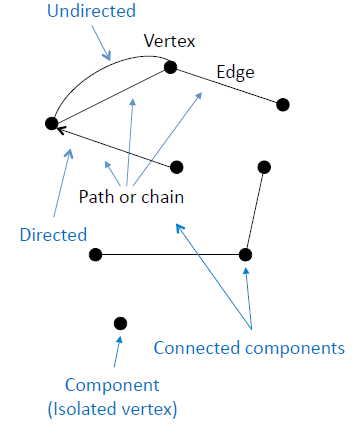
\includegraphics[width=0.4\textwidth]{../Figures/generalGraph.png}
\end{tabular}
\caption{\label{fig:generalGraph} General graph \cite{audestad}.}
\end{figure}


\section{Random Graphs}
Cyber-insurance cover many fields, from financial transactions and outsourcing of tasks to computer networks, many of these fields share a common characteristic, they can all be described as a graph, and often a random graph. Therefore the study of random graphs are of special concern. The research on random graphs are fairly new compared to other mathematical discoveries. E-R graphs were first studied in 1959 by Erdös and Rényi, later and probably with more promising results was the graphs studied by Albert-Barabási in 1999 \cite{audestad}. 
\subparagraph{Erdös-Rényi Graphs}
E-R graphs is a network created between a fixed number of $n$-nodes, where each node connects to another of the $n-1$ nodes with 
probability $p$. The resulting graph will on average contain $n(n-1)p/2 \approx n^{2}p/2$ edges \cite{barabasi}. 
By analysing the graph, the authors found some interesting properties:

\begin{itemize}
\item If $p<n^{-2}$  then there is no edges in the graph. 
\item If $p=c/n$ where c is a constant between $1 < c < log\: n$, the graph will provoke a single large component to grow within the graph.
\item If $p>(ln\: n)/n$ then the graph is completely connected. 
\item If $p = 1/n$ triangles start forming in the graph. 
\end{itemize}

A fully connected E-R graph will have a short diameter similar to the Internet, and thus could be a very good desrcription of the internet. However, the edge degree follows a Poisson distribution, which means that the edge degrees are peaking around the average value \cite{audestad}. Consequently E-R graphs does not capture the immense clustering coefficient which is present in networks such as the Internet. In other words, E-R graphs are not small world graphs, and another graph structure is needed to model computer networks.
A interesting fact about these graphs are their vulnerability, these graphs are very vulnerable against random attacks, such as nature disasters, but robust against directed attacks. Due to the fact that if you remove all edges from one node, it does little damage, since the network is not dependent on single nodes, every node has approximately the same node degree, and it is the sum of all the nodes connections that creates the network.

\subparagraph{\label{ABgraph}Albert-Barabási Graphs}
The structure which is believed to be most accurate regarding modeling computer networks are A-B graphs. A-B graphs are different from E-R graphs since they are scale-free, meaning that the vertices does not have an constant value throughout the entire graph. The formation of an A-B graph results in multiple hubs with a high edge degree. Albert and Barabási found that the edge degree of each vertex follows a power law distribution; meaning that the probability that the edge degree is $g$ is proportional to $g^{\gamma}$
where $\gamma$ usually is a number between 2 and 3 \cite{audestad}. Consequently there are relatively high probability that there exists some nodes that have a very high edge degree. 
These graphs are in contrast to E-R-graphs, very vulnerable to directed attacks, because if you take out a hub, you suddenly destroyed the whole graph. But the graph is very robust against random attacks, this is why most of the networks we observe in the nature can be depicted as A-B-graphs.
A-B graphs can grow and become scale-free if every new vertex is connected to one or more already existing node with a probability proportional to the edge degree of that node . The paper presents an algorithm that creates A-B graphs and figure \ref{fig:ABgraphcreation} shows one graph that evolved from this algorithm:

\begin{itemize}
\item A new single vertex is added to the graph.
\item This vertex is connected to exactly two other vertices in the graph.
\item The probability that the new vertex connects to another vertex is dependent on the edge degree of the other vertex, higher edge degree meaning higher probability
\item There is only one edge between two vertices.
\end{itemize}


\begin{figure}[h]
\centering
\begin{tabular}{@{}c@{}}
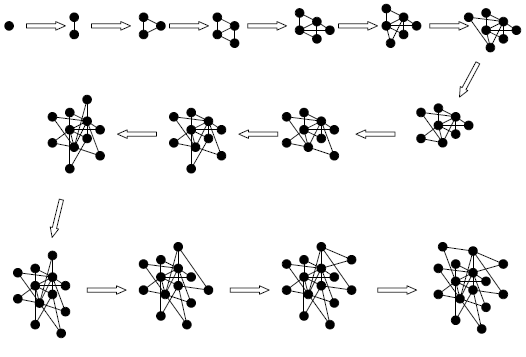
\includegraphics[width=0.8\textwidth]{../Figures/ABgraphcreation.png}
\end{tabular}
\caption{\label{fig:ABgraphcreation} Forming a A-B graph in 15 generations \cite{audestad}.}
\end{figure}

In addition to the high clustering coefficient they showed that A-B-graphs have a fairly small diameter,
 which can be seen in figure \ref{fig:ABgraphcreation}. 
 A-B graphs are therefore comparable to the network formation of the Internet and other computer networks. 
 
\section{Real world graph structures}

The internet, the World Wide Web, neural networks, scientific referencing and co-authorship, stock markets, airline routes, food 
webs, and modular software systems, all tend to evolve in a way similar to that described in the examples 
above. This section will provide some real world examples of how complex systems with huge amount of data can be described as network structures having the same characteristics as A-B graphs.
\subparagraph{Stock markets} The research paper: \cite{greekStockMarket}, analyzes the correlation between different stocks in the Greek stock market in year 1997. They compared the daily closing price of stock $i$ at day $t$, and compared the similarity of a pair of stocks $i$ and $j$ by using the correlation coefficient. The idea is that the correlation coefficient between a pair of stocks can be expressed using different distances in a graph structure. A short distance means high correlation and long distance means low correlations between the stocks. Normally this network would be shown as a fully connected graph, which will consist of $\frac{n(n-1)}{2}$ edges, and would be difficult to analyze. However the approach taken in the paper will present a clear understandable graph consisting of $(n-1)$ edges.

The resulting graph can be seen in figure \ref{fig:greekStockMarket}, and show a network consisting of several clusters linked together. Instead of having to analyze a complex system with huge amount of data, this stock market can be analyzed by its topological properties, such as the high clustering coefficient, i.e a star-topology, which will among others point out which stocks have the most influence on others. 
\begin{figure}[h]
\centering
\begin{tabular}{@{}c@{}}
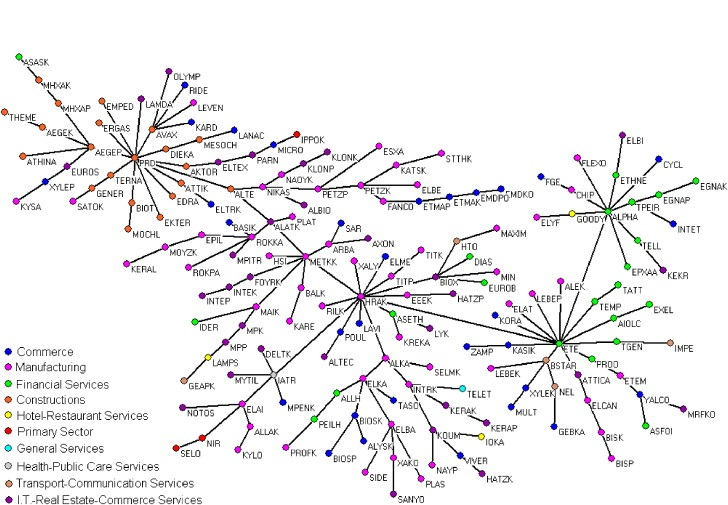
\includegraphics[width=1.0\textwidth]{../Figures/greekStockMarket.jpg}
\end{tabular}
\caption[Caption for LOF]{Network obtained by comparing two stocks correlation coefficient in the Greek stock market (Athens Stock Exchange, ASE) in year 1997. The different colors represent the different sectors of economic activity \cite{greekStockMarket}.
\label{fig:greekStockMarket}}
\end{figure}

\subparagraph{Airline routes}
Another real world network which shows the same characteristics as scale-free graphs is the map of airline routes. Figure \ref{fig:airlineRouteMap} shows the US route map of the American airline company, SkyWest. The characteristic clustering emerges in the figure, where a majority of the flights departs from either Denver, Chicago or San Francisco. Not surprisingly, these airports are all in the top 7 busiest airports in the US \cite{busiestAirports}, and serves as hubs for many of SkyWest flights. In the airline industry some airports are called hubs, because that's what they are, - a connection point for major parts of the network of flights. The network of flights, as depicted \ref{fig:airlineRouteMap} follows the characteristics for A-B graphs. From the graph, we see that the network are vulnerable against direct attacks, meaning if an low edge degree airport is shut down, there will be little consequence for the rest of the network. However, if one of the hubs is forced to close, it will provoke huge delays through out the whole network of flights, because many of the destinations are interconnected via the hubs. 


\begin{figure}[h]
\centering
\begin{tabular}{@{}c@{}}
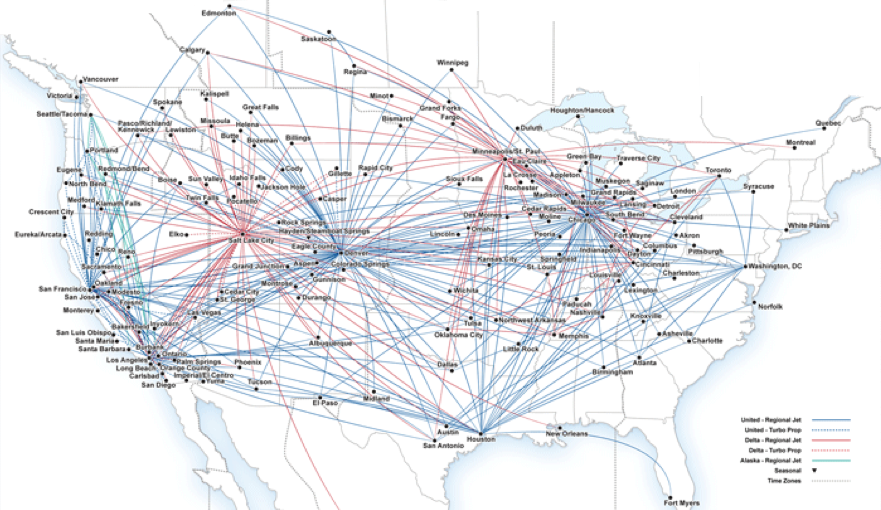
\includegraphics[width=1.0\textwidth]{../Figures/airlineRoutesUSA.png}
\end{tabular}
\caption[Caption for LOF]{SkyWest Airline combined route map \cite{airlineRoutes}.
\label{fig:airlineRouteMap}}
\end{figure}

Similar findings will appear in the different networks mentioned earlier in this chapter, and all of them will experience large consequences if a hub in the network stop functioning. This is important for cyber-insurance because many of the networks we are analyzing tends to look and behave like A-B graphs. For example, transactions between companies, big companies probably have more transactions than small companies, and thus creates a hub, this can be compared with how the correlation between stocks in a stock market works. I.e. we can say that small firms correlate highly with big-firms. 
\chapter{Evolutionary dynamics on graphs}
\label{chp:nature} 


In our paper an insurable topology, is an network structure which makes it feasible for both the
 insurer(supply side)  to offer and the customer(demand side) to acquire insurance.
 For this to be possible there are many  difficulties to overcome,  since risks are correlated, 
 one problem is for the insurer to be able to calculate the overall probability of casualty/infection.
 The paper \cite{lieberman2005evolutionary} is about evolutionary dynamics and how certain structures
can amplify or sustain evolution or drift. This is very usefull for our study of insurable topology, if one
can determine some structures, where certain nodes have certain properties, and these structures
then will sustain viruses from spreading, or amplify the incentive for obtaining cyberinsurance and
antivirus, then we can possibly determine if it is an insurable topology.

In the \cite{lieberman2005evolutionary} paper, they show that advantageous mutant inserted in to a
 circulation graph, will have a fixation probability equal to
\begin{equation}  p_{1}=\frac{(1-1/r)}{(1-1/r^{N})} \label{eq:fixation} \end{equation}
A circulation graph is a graph that satisfy these two properties:
\begin{enumerate}
\item the sum of all edges leaving a vertex is equal for all vertexes
\item the sum of all edges entering a vertex i equal for all vertexes
\end{enumerate}
The fixation probability determines how probable it is that the whole network will eventually be
"infected" by the mutant. I.e. it determines the rate of evolution, which relies on both the size of the
network and the evolution speed. 
A probability equal to one means that every node in the network eventually will be affected by the mutant.

The important question that this paper answer, is if it is possible to find graphs with fixation probability that exceeds \ref{eq:fixation}?, and if so, is it possible to suppress drift and amplify selection or visa versa?
\begin{figure}
\centering
\begin{tabular}{@{}c@{}}
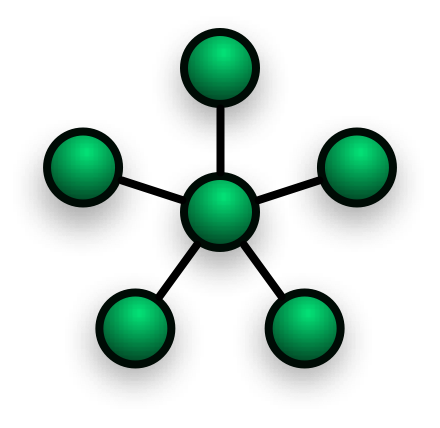
\includegraphics[width=0.5\textwidth]{NetworkTopology-Star.png}
\end{tabular}
\caption{\label{fig:star} A star-topology \cite{lieberman2005evolutionary}. }
\end{figure}

The paper shows that in certain graphs this is possible, one example is the star topology \ref{fig:star}.
In this topology the fixation probability is\begin{equation}p_{2}=\frac{(1-1/r^{2})}{(1-1/r^{2N})} \label{eq:fixation2} \end{equation}.
or more generally: \begin{equation}
p_{k}=\frac{(1-1/r^{k})}{(1-1/r^{kN})} \label{eq:fixationk}
\end{equation}
And as we see when comparing \ref{eq:fixation} and \ref{eq:fixation2} the selective difference is
 amplified from $r$ to $r^{2}$, i.e. a star act as an evolutionary amplifier, favoring advantageous
  mutants and inhibiting disadvantageous mutants.
  
When applying this to our scenario, cyber insurance and insurable topologies, we can use this to show
 that if the center node is strongly secured, then the virus will be considered as disadvantageous and
it will be inhibited from fixation with a certain probability. 
This makes the overall risk easier to calculate for both the insurer and the nodes,
and makes it possible and easier to calculate fair and affordable premiums. 
It can also be used as an incentive for the center node to buy insurance or security software, 
because it can easily be shown how probable an infection will occur. 

One could for example force the center node to buy sufficient anti virus, 
by informing it about how likely it will be infected, and how expensive the cyber insurance will be if 
it do not invest sufficiently in self protection. This will make the whole network more secure, 
and the insurer can now offer insurance to the leaf nodes for a fair price with a calculable risk. 
This could also be used to show how information about cyber-insurance or protection software will
spread throughout a network, and if the information is advantageous, eventually all nodes will acquire
the insurance or software.
    
There are other graphs where the fixation probability is equal to \ref{eq:fixationk}, funnel and
metafunnel. And as we know from the (Kapittel om scale-free and naturlige nettverk) there are many
toplogies in our society that are similar to these graphs.  In all of these, it can be
shown that if N is large enough, the fixation probability for advantageous mutant converges to 1, 
and for disadvantageous converges to 0.

\subsection{Network games}
In the paper \cite{networkgames} they show how network games evolve when the payoffs are determined not only by your own decisions, but also by your neighbours. 
A game that is applicable to our scenario is when considering security software, 
security software can be considered as a public good, it suffers from strategic substitutes, i.e. 
that if your neighbour acquire it, it gives you less incentive to also acquiring the software. 
Public goods and security also benefits from positive externalities, when one acquires the software, 
all the neighbours benefits from it, because the risk of being infected decreases.
Lets consider a simple game shown in this paper.
We have an action space: $X=\{0,1\}$, where 1 can be considered as acquiring information, take vaccine, buy security software etc. And 0 is not doing so.
Each node $i$ has a set of neighbours: $N_{i} $ and a payoff function $y_{i}=x_{i}+\bar{x}N_{i}$
The gross payoff of the game is 1 if $y_{i}>=1$ and 0 otherwise. There is a cost of choosing the action 1, and the cost is: $0<c<1$.
%% [location]h-here, t top, b bottom.
\begin{figure}[h]
\centering
\begin{subfigure}{.4\textwidth}
  \centering
  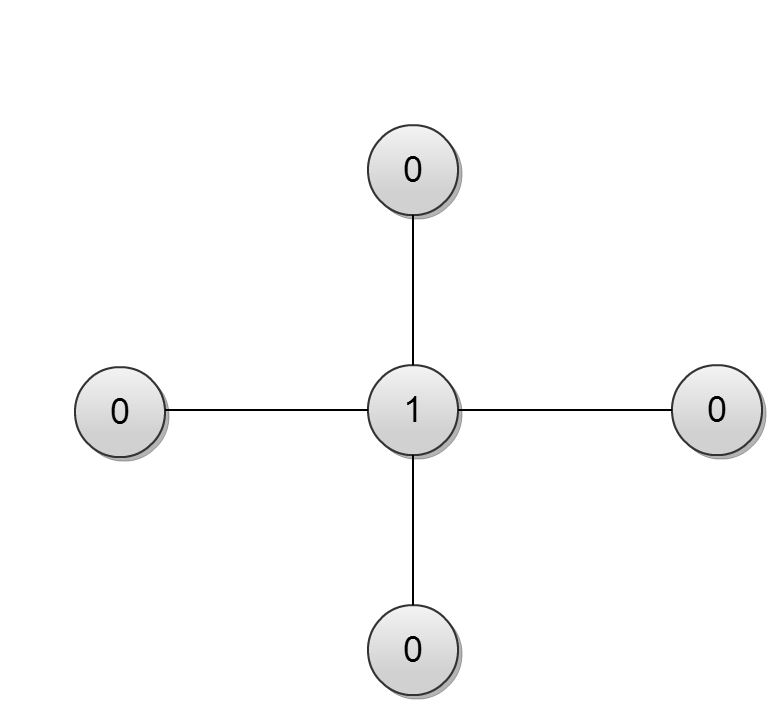
\includegraphics[width=0.8\linewidth]{optimalequilibrium.png}
  \caption{\label{fig:optequi} Socially Optimal equilibrium, center node choose action 1}
\end{subfigure}
\quad
\begin{subfigure}{.4\textwidth}
  \centering
  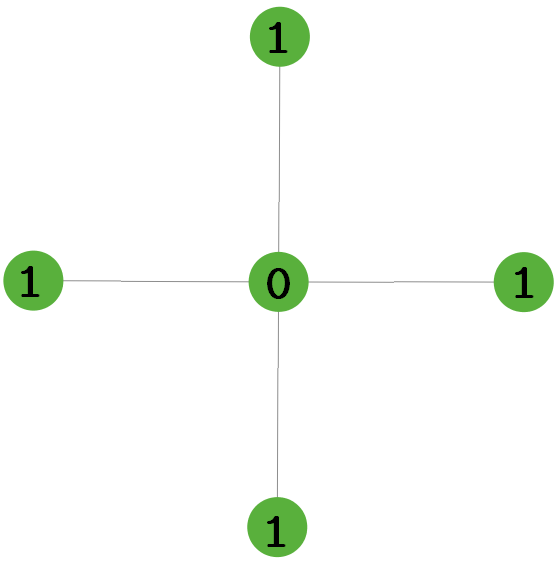
\includegraphics[width=0.8\linewidth]{notoptimalequilibrium.png}
  \caption{\label{fig:notoptequi} Non Socially Optimal equilibrium, leaf nodes choose action 1}
\end{subfigure}
\caption{\label{fig:starequi} Figure \ref{fig:optequi} shows the socially optimal equilibrium, and \ref{fig:notoptequi} shows the non optimal equilibrium.}

\end{figure}

 When we look at the star example, we easily see that there is two equilibriums \ref{fig:starequi}, one where the center node choose action 1 and the rest of the nodes choose action 0, and a second equilibrium where all the leaf nodes chooses 1 and the center choose 0.
The overall payoff in these two differ from each other, the latter is not socially optimal because it
 suffers from a cost equal to: $\#leaf nodes*c$ versus the first equilibrium where the total cost is only $c$.
If we could have forced to network game to end up in the socially optimal equilibrium, this would have been optimal. 
One possibility could be for the insurer to offer cheap insurance to all the leaf nodes, and a expensive one to the center node. By expensive we mean a cost that exceeds the cost of acquiring self protection, because then a rational center node would striclty prefer buying security software, as long as the price for acquiring and maintaining it is less than the possible cost of loss.
\begin{equation}
 U_{center}=-Probability_{casualty}*\alpha-Cost_{selfprotection}
 \label{eq:utility}
 \end{equation} 
A risk averse player would like to maximize her expected utility \ref{eq:utility}. We assume that the probability of casualty is significantly smaller when acquiring self protection, versus not acquiring. If the options for a player is
 either to remove the expected loss of casualty by acquiring self protection, or by insuring against it,
and the expected utility of acquiring insurance is lower than the expected utility of acquiring self protection. The player would strictly prefer self protection. 
This is one possible way of forcing the network game to end up in an insurable star topology.
//
Thoughts on what this fixes in a simple way...
The insurer can now calculate the probability for catastrophic event(all nodes suffer), and now atleast has a measurement on the correlated risk. It has also limited the information asymmetry to concern only one node, the center node. It does not matter if the leaf nodes acquire security or not. Also it has now limited the interdependent security to one node, the center node.

//
//
 notater:
 
The game:
The way this game works, is that we look at nodes that are mutated (A), and those who are not (B).  
\begin{table}[h]
\centering 
\begin{tabular}{ l | c | r }
  
   & A & B \\  \hline  
  A & a & b \\ \hline  
  B & c & d \\
  
\end{tabular}
\caption{\label{fig:gamesetup} Setup propagation game \cite{lieberman2005evolutionary}}
\end{table}

When we apply the game to a directed graph, there are four different outcomes, a,b,c and d, which represents the interaction between the nodes, as is depicted in the figure below\ref{fig:game}. 

In the first figure (Positive symmetric) the fixation probability is related to r=b/c. If b is greater than c, the properties of mutant b will propagate in to all the other nodes, and the whole graph will eventually consists of only mutated nodes. The opposite will happen in the case where c is greater than b, leading to extinction of the mutation. The later scenario models the situation where proper protection against a mutant i.e. a security threat is installed. If the level of security, c is higher that the strength of the security threat it will be blocked from propagating further into the network. 


\begin{figure}[h]
\centering
\begin{tabular}{@{}c@{}}
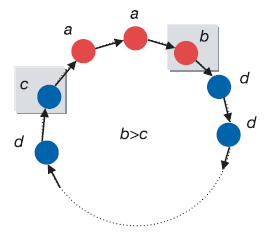
\includegraphics[width=0.5\textwidth]{natureGameSingle.png}
\end{tabular}
\caption{\label{fig:game} Mutant propagation game}
\end{figure}


More generalized, $W$ does not need to be stochastic, $w_{ij}>=0$. 
If the sum of all edges leaving a vertex is equal for all vertexes, then the graph will never suppress selection.
If the sum of all edges entering a vertex is equal for all vertexes, the graph never suppress drift.
If both then the graph is called a circulation.
     
To be able to point out insurable topologies, an extensive study of different graphs and how they behave has to be conducted. Regarding security, knowledge of how viruses spread and how to use graph structures to prevent malicious hackers from entering your network is important. Evolutionary dynamics, and the research of how mutant genes spread though out a population fits in to the model of security. 

Where the fixation probability determines the rate of evolution, which relies both on the size of the network and the evolution speed. A probability of 1 means that every node in the network eventually will be affected by the mutant.   
Isotherm graphs are a sub-graph of circulation. 

If $W$ is symmetric, or isotherm then the fixation probability is always \ref{eq:fixation}
isotherm means doubly stochastic, all rows and cols sum to 1. 
If a graph is one rooted, it has a fixation prob of $1/N$ regardless of $r$. If a graph has more then one root, its fixation probability is zero. 
Is it possible to find graphs with fixation probability that exceeds \ref{eq:fixation}? Is it possible to suppress drift and amplify selection?

And the selective difference is as we see amplified from $r$ to . i.e. a star act as an evolutionary amplifier,
 favoring advantageous mutants and inhibiting disadvantageous mutants, tilts towards selection and against drift.
 
 
 in certain graphs, star, funnel, metafunnel, if N is large enough, fixation probability for advantageous mutant converges to 1. Fixprob for disadvantageous converges to 0.
 
 
The same theory can be used to demonstrate how the aggregated security of a network is higher if the central node of a star structure is secured. 
If we assume that implemented security is 100$\%$ efficient, no threats will propagate beyond that node i.e total security for the network is increased. 
Scale-free networks have most of their connectivity clustered in a few vertices, i.e. they are potent selection amplifiers.


NOTES!!!
Geek stockmarket graph: http://www.sciencedirect.com/science/article/pii/S037843710700221X



Hvorfor er slike strukturer viktige å forstå for oss? 
Som vi skal se senere oppfører hubene seg i A-B grafene som stjerne-topologier. 
Ved å ha oversikt over sitt eget nettverk vil man kunne identifisere hvor disse stjernene befinner seg, nettopp disse er det viktig at man sikrer for å ungå spredning av virus, samt fungere som en blokkade mot andre trusler e.g. hackers. (TROR DET er viktig at vi prøver å fokusere mot insurable og ikke spredning av virus.)
så noe sånt:
nettopp disse er viktige slik at man lettere kan kalkulere riskioen, og gi insentiver, ved hjelp av cyber insurance, til hubsa for å sikre seg eller no.








\chapter{Methodology}


\section{Graph}
There are some basic properties of graphs which is important to be familiar with. Figure \ref{fig:generalGraph} depicts the basics of an unweighted graph, the edges are not assigned any value. Weighted edges can be useful to e.g. reflect capacity constraints such as a link's maximum bandwidth, or the length of a road(edge). Other common definition used when describing graphs are listed below \cite{audestad}:
\begin{itemize}
\item Edge degree: Number of edges connected with a node.
\item Hub: Node with high edge degree.
\item Cycle: A chain originating and terminating at the same node.
\item Cluster: Subgraph of highly connected nodes.
\item Cluster coefficient: Probability that two nodes that are adjacent to a third node are also adjacent.
\item Clique: Subgraph where all nodes are adjacent (cluster coefficient = 1).
\item Small world graph: Graph with small diameter and large cluster coefficient (e.g. the Internet and A-B graphs, described in section \ref{ABgraph}).
\end{itemize}

\begin{figure}[h]
\centering
\begin{tabular}{@{}c@{}}
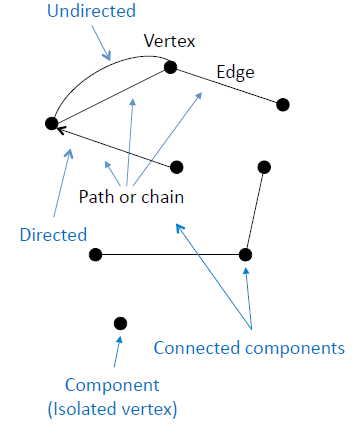
\includegraphics[width=0.4\textwidth]{../Figures/generalGraph.png}
\end{tabular}
\caption{\label{fig:generalGraph} General graph \cite{audestad}.}
\end{figure}


\section{Random Graphs}
Cyber-insurance cover many fields, from financial transactions and outsourcing of tasks to computer networks, many of these fields share a common characteristic, they can all be described as a graph, and often a random graph. Therefore the study of random graphs are of special concern. The research on random graphs are fairly new compared to other mathematical discoveries. E-R graphs were first studied in 1959 by Erdös and Rényi, later and probably with more promising results was the graphs studied by Albert-Barabási in 1999 \cite{audestad}. 
\subparagraph{Erdös-Rényi Graphs}
E-R graphs is a network created between a fixed number of $n$-nodes, where each node connects to another of the $n-1$ nodes with 
probability $p$. The resulting graph will on average contain $n(n-1)p/2 \approx n^{2}p/2$ edges \cite{barabasi}. 
By analysing the graph, the authors found some interesting properties:

\begin{itemize}
\item If $p<n^{-2}$  then there is no edges in the graph. 
\item If $p=c/n$ where c is a constant between $1 < c < log\: n$, the graph will provoke a single large component to grow within the graph.
\item If $p>(ln\: n)/n$ then the graph is completely connected. 
\item If $p = 1/n$ triangles start forming in the graph. 
\end{itemize}

A fully connected E-R graph will have a short diameter similar to the Internet, and thus could be a very good desrcription of the internet. However, the edge degree follows a Poisson distribution, which means that the edge degrees are peaking around the average value \cite{audestad}. Consequently E-R graphs does not capture the immense clustering coefficient which is present in networks such as the Internet. In other words, E-R graphs are not small world graphs, and another graph structure is needed to model computer networks.
A interesting fact about these graphs are their vulnerability, these graphs are very vulnerable against random attacks, such as nature disasters, but robust against directed attacks. Due to the fact that if you remove all edges from one node, it does little damage, since the network is not dependent on single nodes, every node has approximately the same node degree, and it is the sum of all the nodes connections that creates the network.

\subparagraph{\label{ABgraph}Albert-Barabási Graphs}
The structure which is believed to be most accurate regarding modeling computer networks are A-B graphs. A-B graphs are different from E-R graphs since they are scale-free, meaning that the vertices does not have an constant value throughout the entire graph. The formation of an A-B graph results in multiple hubs with a high edge degree. Albert and Barabási found that the edge degree of each vertex follows a power law distribution; meaning that the probability that the edge degree is $g$ is proportional to $g^{-\gamma}$
where $\gamma$ usually is a number between 2 and 3  This distribution is called a thick-tail distribution, because there is a significant probability that a node may have a very high degree. \cite{audestad}
These graphs are in contrast to E-R-graphs, very vulnerable to directed attacks, because if you take out a hub, you suddenly destroyed the whole graph. But the graph is very robust against random attacks, this is why most of the networks we observe in the nature can be depicted as A-B-graphs.
A-B graphs can grow and become scale-free if every new vertex is connected to one or more already existing node with a probability proportional to the edge degree of that node . The paper presents an algorithm that creates A-B graphs and Figure \ref{fig:ABgraphcreation} shows one graph that evolved from this algorithm:

\begin{itemize}
\item A new single vertex is added to the graph.
\item This vertex is connected to exactly two other vertices in the graph.
\item The probability that the new vertex connects to another vertex is dependent on the edge degree of the other vertex, higher edge degree meaning higher probability
\item There is only one edge between two vertices.
\end{itemize}


\begin{figure}[h]
\centering
\begin{tabular}{@{}c@{}}
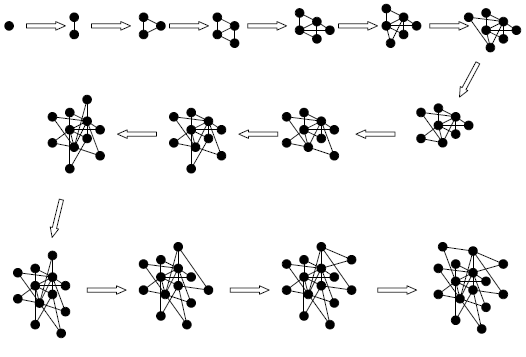
\includegraphics[width=0.8\textwidth]{../Figures/ABgraphcreation.png}
\end{tabular}
\caption{\label{fig:ABgraphcreation} Forming a A-B graph in 15 generations \cite{audestad}.}
\end{figure}

In addition to the high clustering coefficient they showed that A-B-graphs have a fairly small diameter,
 which can be seen in Figure \ref{fig:ABgraphcreation}. 
 A-B graphs are therefore comparable to the network formation of the Internet and other computer networks. 






\section{Game Theory}
Here we will present some of the game theory concepts we use in our models, for more thoroughly explanation of game theory, see: \cite{nisan2007algorithmic}.
\subparagraph{One shot game}
This type of game assumes that players act at the same time instant, therefore there is no causality. A game in strategic (normal) form can be described by three elemetns:
\begin{itemize}
\item the set of players $i \in I$, which we take to be the finite set ${1,2,....,I}$.
\item the pure-strategy space $s_{i}\in S_{i}$ for each player i, where $s_{i}$ is a possible action of player i.
\item and payoff functions $U$, which gives the players utility functions for each profile $s=(s_{1},s_{2},...,s_{I})$ of strategies.
\end{itemize}
A general solution concept for games of economic interest is the Nash Equlibrium solution. A Nash Equilibrium is a profile of strategies such that each players strategy is an best response to the other players strategies. 
\subparagraph{Nash Equilibrium}
A pure strategy profile $s^{*}$ is a Nash eqilibirum if, for all players $i$
\begin{equation}
U_{i}(s^{*}_{i},s_{-i}^{*})\geq U_{i}(s_{i},s^{*}_{-i}) \in S_{i}
\end{equation}
\subparagraph{Stackelberg}
Also known as a leader-follower game, it introduces multiple stages. The leader commits itself first, chooses its strategy, then the followers respond sequentially. The Stackelberg model can be solved to find the subgame perfect Nash Equilibrium, i.e. the strategy profile that serves each player best, given the strategies of the other players and that entails every player playing in a Nash Equilibrium in every subgame.
\subparagraph{Subgame-perfect equilibrium}
A strategy profile $s$ is a subgame perfect equilibrium if it represents a Nash Equilibrium of every subgame of the original game.
\subparagraph{Socially optimal}
A socially optimal outcome is the set of choices that maximizes the sum of all players payoffs. 
\subparagraph{Price of stability}
The price of stability (PoS) of a network game, is the ratio between the maximum sum of the players payoff, in a stable outcome, and the Socially optimal outcome.

\subparagraph{Bayesian game}
In Bayesian games, information about the other players characteristics is incomplete. In these types of games, there are one player(the agent) who knows both types, and another player (the principal) who does not know the type of the other player. 

A pooling equilibrium, is a equilibrium where all both types of the agent chooses the same action, i.e. the principal is not able to distinguish the two types. 
A separating equilibrium is an equilibrium where the agents of different types, choose different actions, and thus the principal is able to determine the agents type by observing his actions.


\section{Netlogo}
In addition to analyzing the different models with game theory, we created a simulator for the models, in a program called Netlogo. Netlogo is a programmable modeling environment for simulating natrual and social phenomena. It is well suited for modeling complex systems developing over time \cite{netlogo}.
Netlogo where good to model our complex network formation games, and at the same time provided us with a good graphical user interface, that enabled us to see the result of the games, and also to easily adjust the different parameters.
In Figure \ref{fig:netlogo} we see the user interface, which are used to setup the parameters, start the modeling, and showing the resulting network formation. Figure \ref{fig:netlogo-code} shows how the coding interface looked like. For detailed overview of the code used in our different models, see the appendix.
\begin{figure}[h]
\centering
  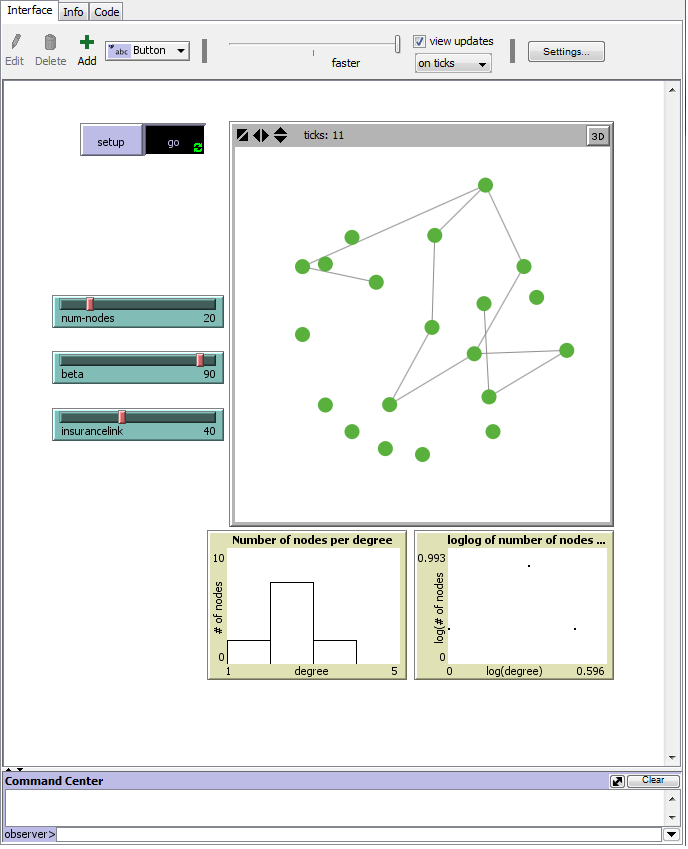
\includegraphics[width=0.9\linewidth]{../Figures/netlogoexample.png}
  \caption{\label{fig:netlogo} The figure shows a screen capture of netlogo, while we are running one of our simulations.}

\end{figure}
\begin{figure}[h]
\centering
  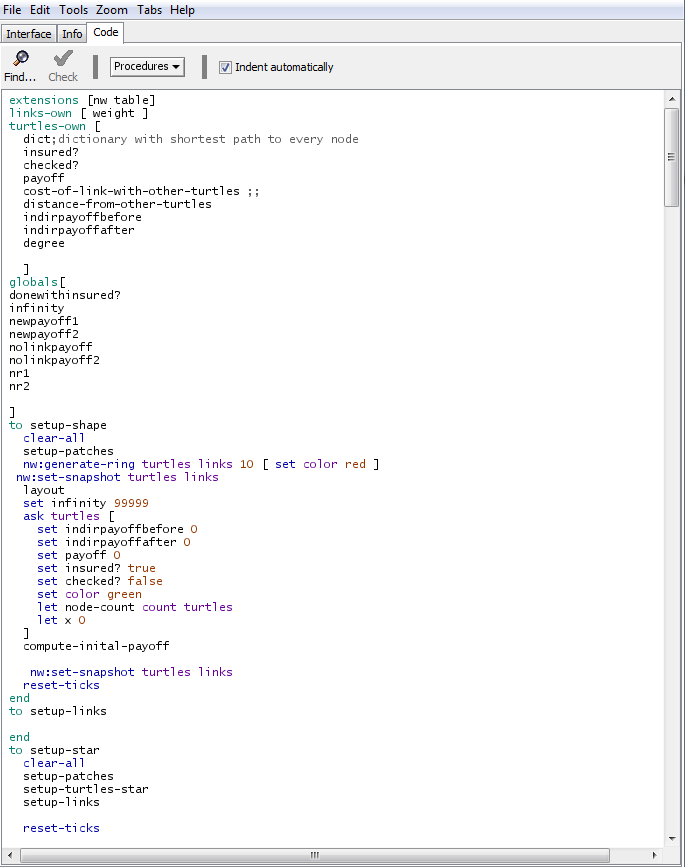
\includegraphics[width=0.9\linewidth]{../Figures/netlogocodeexample.png}
  \caption{\label{fig:netlogo-code} The figure shows how the code interface in netlogo looks like.}

\end{figure}





%Part 2: Contributions/Modelene vaare

\chapter{Modeling Cyber-Insurance }
\label{chp:modelingCyberInsurance} 


\section{Network Formation}


In many scenarios agents seeks to create networks in order to directly benefit from each other. The established links might represent companies out sourcing part of their manufacturing, or cooperative agreements in the development of new software products. In addition to increase the trade-off, each of the established links represents risk of being a victim of cascading failures. The intuitive example is the spread of epidemic diseases, also  (node failures of a power grid and) financial contagion such as the one back in 2008 was a result of cascading failures. Strategic network formation using cyber-insurance can be used to prevent such situation in addition to increase the overall payoff of participants in a clustered network.


When deciding whether to establish connection to a neighbour agent, the payoff has to be a balance between the expected earnings and the risk of the other party failing to complete the transaction. This is the reason why we seek to only download content from trusted peers and outlaw MC-gangs are consistently skeptical to enter into new agreements despite promising increased earnings, since the risk of undercover police are too high. 


In the paper \cite{contagion}, they come up with some interesting results regarding network formation games. 
They set up a game where the nodes benefit from direct links, but these links also expose them for risk. 
Each node gains a payoff of  $a$ per link it establishes, but it can establish a maximum of $\delta$ links.
A failure occur at a node with probability $q$, and propagates on a link with probability $p$. If a nodes fail, it will receive a negative payoff of $b$, no matter how many links it has established.

The results from their model shows a situation where clustered graphs achieve a higher payoff when connected to trusted agents, compared to when connecting with random nodes. Unlike in anonymous graphs, where nodes connect to each other at random, nodes in these graphs share some information with their neighbours, which is used when deciding whether to form a link or not. 
To further explain these results, they show that there exists a critical point, called phase transition, which occurs when nodes have a node degree of $1/p$. 
At this point a node gets a payoff of $a/p$, to further increase the payoff the node needs to go into a region with significantly higher failure probability. 
Because once each node establish more than $1/p$ links, the edges which propagates risk, will with high probability form a large cluster. Which results in a rise in probability of node failure, and reduces the overall wellfare.
From this the paper say that when the minimum welfare exceeds 
$(1+f(\delta)*a/p)$
we have reached super critical payoff. Otherwise it is called sub-critical payoff. 
Further they show that the only possible way of ending up with supercritical payoff, is by forming clustered networks consisting of cliques with slightly more than $1/p$ nodes. 
If the nodes form an anonymous market, random linking, they can only get sub-critical payoff. 
In other words, if the nodes can choose who they connect with, and by doing so, creating trusted clustered markets, they can achieve a higher payoff, by exceeding the critical node degree point. But in random graphs, this is not possible. 


Inspired by this model, we created a model which shields light on how cyber-insurance can be used in network formation to prevent cascading failures and increase an agents payoff.  



\section{Very Simple Model}

As a starting point the model is highly simplified in order to show the concept of how cyber-insurance can be used to create an insurable topology. Through out this chapter new features will be added to the model to make it more realistic and applicable. To begin, the model is formulated as follows.
A set of $n$ agents are randomly chosen to be insured or not. They all get their own fixed income, and by connecting to other agents they will receive a benefit resulting in higher payoff. Non-insured agents will have a risk of failure i.e. an expected cost of failure. Therefore if an insured agents chooses to connect to a non-insured agent they will also suffer from this expected cost of failure. In other words, the model follows a rule that insured agents are only willing to connect to other insured agents and non-insured agents can only connect with each other. In addition we apply the assumption that each node goes through the whole graph to decide whether to establish a connection or not. Since the decision is bidirectional, i.e. each agent must agree to establish the connection, the resulting graph will always be two fully connected cliques, one consisting of a insured agents and the other of non-insured agents. 


This dichotomy represents a trusted environment for the insured nodes, because they are able to trust each other since everyone is protected from risks such as financial catastrophe. These agents will benefit from each connection without having to worry about contagious risks from the connected agents. 
An agent in the non-insured clique will also receive the aggregated benefits from the connections, however each of the connection has a probability of failure. Hence this environment is not trusted, and a decision on whether to connect always involves some risks. 

\begin{figure}[h]
\centering
\begin{subfigure}{.5\textwidth}
  \centering
  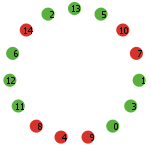
\includegraphics[width=0.4\linewidth]{../Figures/firstModelWithNoParameters1.png}
  \caption{\label{fig:firstmod1} 15 Agents randomly choosen to be either insured (green) or non-insured (red.}
\end{subfigure}
\quad
\begin{subfigure}{.46\textwidth}
  \centering
  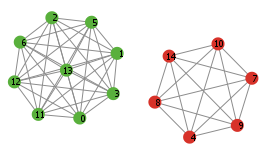
\includegraphics[width=0.8\linewidth]{../Figures/firstModelWithNoParameters2.png}
  \caption{\label{fig:firstmod2} Two clustered networks. One consisting of insured agents the other consists of non-insured.}
\end{subfigure}
\caption{\label{fig:fincont} shows how insured agents connects with each other to form a network to achieve super-critical payoffs.}
\end{figure}

In many situations agents, such as companies are in a situation where they have to establish connections. One example can be a non-insured company needing to outsource certain tasks to remain competitive, if all the potential companies for outsourcing are insured, the company will have a strong incentive to also buy insurance in order to be able to establish a connection. Hence this model, although very simple, shows an insurable topology where insured agents benefit from being insured. 

There are some limitations of the model, among others it fails to reflect the dynamics of a real world scenario, where each node will have different variables with different values. In addition, each node have a complete overview of the other nodes status. i.e. the problem with information asymmetry is not taken into account. 

\subsection{Model with parameters}
To make this simple model more realistic, we have to create a game with parameters, The characteristics of the game is as follows: an agent can be either insured or not insured, the insured ones have to pay an insurance cost $I_{0}$. Every agent starts with a fixed income, $\alpha$, to further increase their income they have to establish links to other agents. For each link they establish they receive a payoff of $\beta$. An insured node has to pay a cost of $I_{l}$ for every link he establish. The game is bidirectional, so both agents has to agree to the establishment of a link, and if both are insured, they both have to pay the cost $I_{l}$. 
Every agent who is not insured will have a risk of failure(infected, bankruptcy, or some other type of failure), this is captured with the expected risk cost $r$. Every node who connects to an node who is not insured will also suffer from this cost. See Table \ref{tbl:simplegamepara} for an overview of the parameters. 
\begin{table}[h]
\centering
\begin{tabular}{lc}
 \hline
  $\alpha$ - agents fixed income\\
  $\beta$ - income from establishing a direct link \\
  $I_{o}$ - cost of having insurance. \\
  $I_{l}$ - increased insurance cost per link the node establishes\\
  $r$ - expected risk cost\\
  \hline
\end{tabular}
\caption{Table showing the parameters to be used in the first model \label{tbl:simplegamepara}}
\end{table}
\subparagraph{Two agent game}
To begin analysing this game, lets consider a two-person game at first. In this game the strategy space of both players consist of four different strategies. They can choose insurance or not, and to establish link or not. I.e. the different strategies are: be insured and establish link noted as: $IL$, 
be insured and do not establish link: $I\overline{L}$. Not insured and establish link: $\overline{I}L$, and not insured and do not establish link: $\overline{IL}$.
Figure \ref{fig:FirstGameTheoryModel} shows the different outcomes of this game.

\begin{figure}[h]
\centering
\begin{tabular}{@{}c@{}}
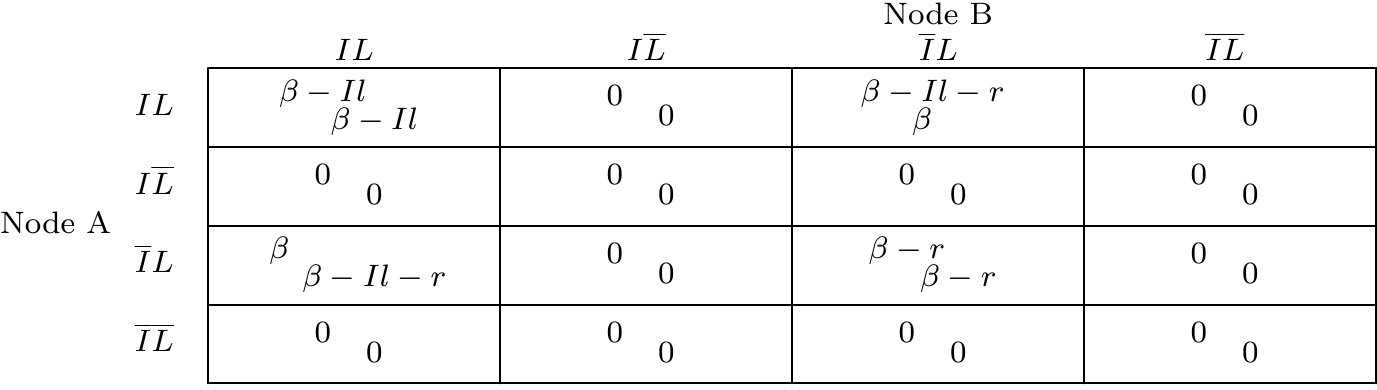
\includegraphics[width=1.0\textwidth]{../Figures/FirstGameWithParameters.png}
\end{tabular}
\caption{\label{fig:FirstGameTheoryModel} Normal form game, showing the different strategies and the payoffs  for the different outcomes. The payoff for agent A is written first, then the payoff for agent B is on the line beneath.
 An agent has a strategy space of size 4. }
\end{figure}

The simple game described earlier where the insured nodes form a trusted clique is what we want to achieve. 
When non-insured nodes connect to each other, they both end up with this payoff \ref{eq:notinsured payoff}. If they do not establish connection, they both receive the payoff \ref{eq:notinsured payoff2}.
\begin{equation}
U_{i}=\alpha - 2*r +\beta
\label{eq:notinsured payoff}
\end{equation}
\begin{equation}
U_{i}=\alpha - r
\label{eq:notinsured payoff2}
\end{equation}
From this equation we see that if $r>\beta$ then no connections will be made between non-insured agetents, because then they would strictly prefer the payoff from not connecting.
If a insured agent connects to an non-insured one, he will end up with this payoff \ref{eq:insured-noninsured}. If he dont connect he will receive this payoff \ref{eq:insured-noninsured2}.
\begin{equation}
U_{i}=\alpha - I_{0} - I_{l} - r + \beta
\label{eq:insured-noninsured}
\end{equation}
\begin{equation}
U_{i}=\alpha - I_{0}
\label{eq:insured-noninsured2}
\end{equation}
As we see if $I_{l}+r>\beta$ the insured one will prefer not to connect, if not he will establish connection, and since the non-insured agent is always better off when connected to an insured agent, he will accept the establishment. This is easy to see when comparing the two payoffs. Payoff of connecting to a insured one: $U_{i}=\alpha - r + \beta$ is allways higher than not connecting: $U_{i}=\alpha - r$ this holds as long as $\beta>0$.
To ensure that only insured nodes connect to each other, we want \ref{eq:insured-noninsured2} to be larger than \ref{eq:insured-noninsured}. I.e. This has to hold:
\begin{equation}
I_{l}+r>\beta
\label{eq:condition}
\end{equation}
When insured nodes connect to other insured nodes, they both end up with this payoff:
\begin{equation}
U_{i}=\alpha - I_{0} - I_{l} + \beta
\label{eq:insured-insured}
\end{equation}
To ensure that both agents will connect to each other this has to hold:
 \begin{equation}
I_{l}<\beta
\label{eq:condition2}
\end{equation}
For the game to end up as the one described earlier, where only insured nodes connect to other insured nodes, both \ref{eq:condition} and \ref{eq:condition2} has to hold, which gives us this limitation on the parameter $I_{l}$:
\begin{equation}
\beta-r<I_{l}<\beta
\label{eq:final condition}
\end{equation}
For the non-insured nodes to connect to each other, the only condition is that $\beta>r$. As long as these limitation is fulfilled, the game will end up with insured agents only establishing connections to other insured nodes, and non-insured nodes only connecting to non-insured nodes. It is easily seen that this holds for the two-agent game but also when there are multiple agents in the game.

In this model the network formation is done endogenously, and when following the limitation \ref{eq:final condition} we ensure that only insured nodes will connect, and we end up with an insurable network topology. 
In this model we have neglected the information problem, we assume that all nodes can differentiate insured versus non insured nodes. This could be difficult to realize in many real world network, but in financial transactions and in software development networks, it is reasonable to assume that the parties can acquire this type of information regarding their transactional partners. And thus they solve the information asymmetry problem by them self, by requiring proof of insurance prior to establishing a connection. This will result in insurable-clustered components  evolve endogenously in the network. Which is beneficial for both the insurer and the nodes.

\subparagraph{Example scenario}
By assigning values to the variables, we can show the outcome of the game in different scenarios. With the values from \ref{tbl:simplegamevalue}, the insurance cost of establishing a link satisfies the condition in equation \ref{eq:final condition}.
If we play this game between two agents we can see the result in the normal form table:\ref{fig:NFnumbers}. 
We see that the results are as we expected, insured nodes will only choose to connect with other insured nodes, they are also satisfied when not connected to each other, but this is not the social optimal outcome, and since they have complete network information, they will choose to connect to each other, because they will both achieve receive a higher payoff.
As we know, it does not matter if we consider only a two person game, because the change in payoffs when adding a link, is linear an independent of the agents degree, thus no insured agents will connect to non-insured ones.
\begin{table}[h]
\centering
\begin{tabular}{lc}
 \hline
  $\alpha=10,
  \beta=10,
  I_{o}=5,
  I_{l}=3,
  r=8$\\
  \hline
\end{tabular}
\caption{Table showing the parameters and their assigned values \label{tbl:simplegamevalue}}
\end{table}

\begin{figure}[h]
\centering
\begin{tabular}{@{}c@{}}
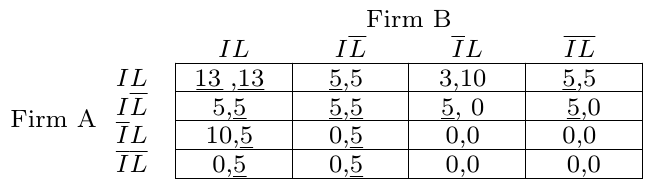
\includegraphics[width=1.0\textwidth]{../Figures/gameTheoryModel1WithNumbers.png}
\end{tabular}
\caption[Caption for LOF]{Normal form game between two agents with the parameters given in \ref{tbl:simplegamevalue}, the best response of a player to a given strategy is marked with an underscore.There are two pure nash equilibriums in this game,$IL,IL$ and $I\underline{L},I\underline{L}$. \label{fig:NFnumbers}}
\end{figure}
When setting the insurance cost: $I_{l}<\beta - r$ or $I_{l}>\beta$ we are violating the condition who ensured that only insured nodes connected to each other. The results are shown in Figure \ref{fig:NFnumbersViolating}. As we see there are still the same nash equilibrium, but whats interesting is the best response of an insured agent when the other agent is not insured, and both choose to establish link. This scenario has now changed, and we see that the insured agent would agree to the link establishment, this could result in an untrusted and thus an non-insurable topology. Therefore to ensure that only insured agents connect to each other, equation \ref{eq:final condition} has to be satisfied. 
In this particular situation with only two agents, the game will still end up in one of the nash equilibriums and only insured will connect to insured. But imagine a situation with more agents, then the insured node will also connect to the non-insured ones, and thus create a non-trusted network(non-insurable topology).
\begin{table}[h]
\centering
\begin{tabular}{lc}
 \hline
  $\alpha=10,
  \beta=10,
  I_{o}=5,
  I_{l}=1,
  r=8$\\
  \hline
\end{tabular}
\caption{Table showing the parameters and their assigned values, the insurance cost of establishing link is now violating the equation \ref{eq:final condition} \label{tbl:simplegamevalue2}}
\end{table}

\begin{figure}[h]
\centering
\begin{tabular}{@{}c@{}}
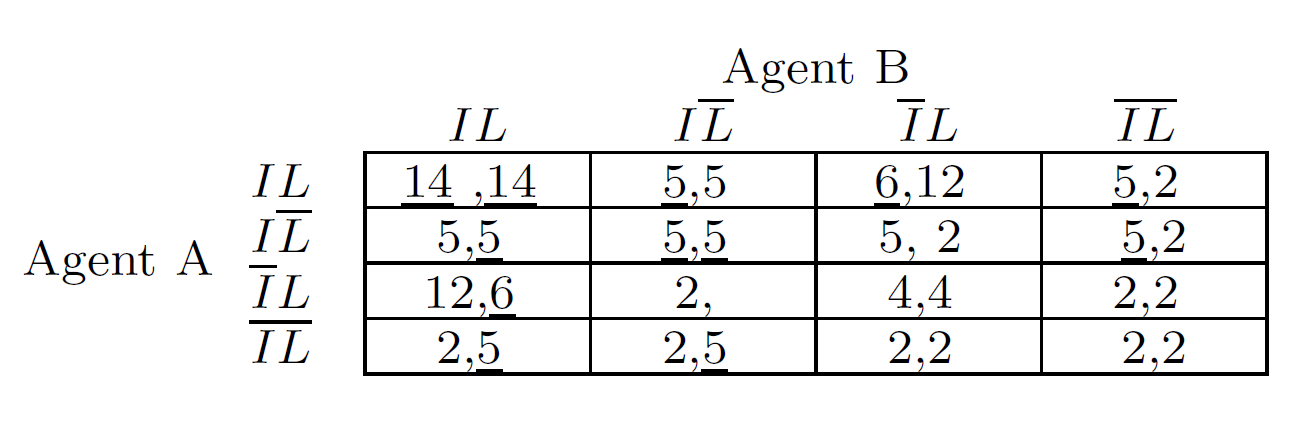
\includegraphics[width=1.0\textwidth]{../Figures/NotOptimalGameWithNumbers.png}
\end{tabular}
\caption[Caption for LOF]{Normal form game between two agents with the parameters given in table \ref{tbl:simplegamevalue2}, the best response of a player to a given strategy is marked with an underscore.There are two pure nash equilibriums in this game,$IL,IL$ and $I\underline{L},I\underline{L}$. \label{fig:NFnumbersViolating}}
\end{figure}



\subparagraph{BRUKE DETTE ET ANNET STED KANSKJE? BLIR LITT RART Å HOPPE INN I DET HER}
By adjusting the parameter one can assure that only insured agents connects to other insured agents, and the opposite,
that only uninsured agents connects to each other. Hence as we can see from the figure \ref{fig:fincont} clustered
networks of insured agents (red) are created, and  as the paper \cite{contagion} showed, these clustered trusted
networks, can achieve higher, super-critical, payoff by increasing their node degree past the critical point.

\begin{figure}[h]
\centering
\begin{subfigure}{.5\textwidth}
  \centering
  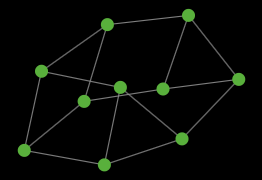
\includegraphics[width=0.8\linewidth]{../Figures/financialContagion1.png}
  \caption{\label{fig:fincont1} Initial graph with 10 agents.}
\end{subfigure}
\quad
\begin{subfigure}{.46\textwidth}
  \centering
  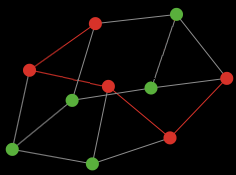
\includegraphics[width=0.8\linewidth]{../Figures/financialContagion2.png}
  \caption{\label{fig:fincont2} Insured agents (red) forms a network}
\end{subfigure}
\caption{\label{fig:fincont} shows how insured agents connects with each other to form a network to achieve super-critical payoffs.}
\end{figure}

, because the nodes can thus receive a super-critical payoff, and they are also insured against contagious risk.  

Figure \ref{fig:GTmodel1equations} presents the individual payoffs in a formation game between two agents in the described model. It is assumed that both agents has to have a desire to establish a connection in order to create a link between them. This is reasonable since a company would not prefer to enter into an agreement with negative expected payoff. As in this case would be the result when an insured agent is requested a connection with someone without insurance. 
 
 
\begin{figure}[h]
\centering
\begin{tabular}{@{}c@{}}
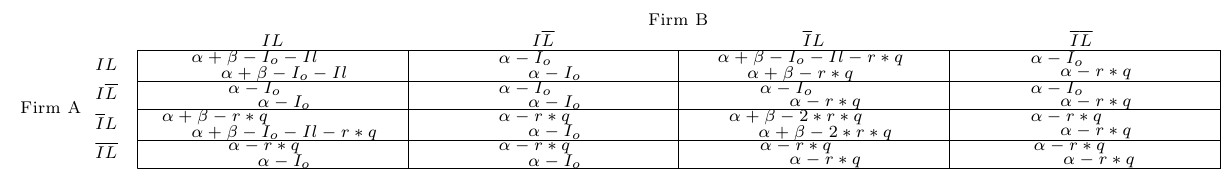
\includegraphics[width=1.0\textwidth]{../Figures/gameTheoryModel1WithEquations.png}
\end{tabular}
\caption[Caption for LOF]{\label{fig:GTmodel1equations} Normal form game between two agents individually choosing to purchase insurance and express desire to connect to the other  \footnotemark }
\end{figure}
\footnotetext{A link will only be created if both agents wishes to establish a connection.}

If we give value to the variables in figure \ref{fig:GTmodel1equations} one can observe the model's different equilibrium's. It is difficult to know exactly how the variables are set and this would vary considerably between different markets. In a real worlds scenario the variables would also be different for each agent. However in figure \ref{fig:GTmodel1} we decided to set a fixed value (which is assumed to be corresponding to the real values) for each variable in order to show a concept of how cyber-insurance can be used to create beneficial payoffs.
The following values where used: $\alpha$ = 10, $\beta$ = 10, $I_{o}$ = 5, $I_{l}$ = 2, $r$  = 20, $q$ = 0.5.


\begin{figure}[h]
\centering
\begin{tabular}{@{}c@{}}
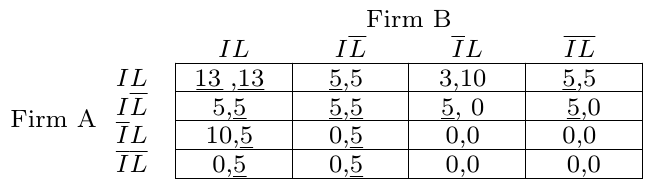
\includegraphics[width=0.6\textwidth]{../Figures/gameTheoryModel1WithNumbers.png}
\end{tabular}
\caption{\label{fig:GTmodel1} Shows equilibrium's in the resulting payoff matrix.}
\end{figure}

From the payoff matrix \ref{fig:GTmodel1} we observe two different Nash equilibrium's: One when both agents are insured and wants to connect to the other agent, and one when both are insured but does not want to establish a connection. These are the possible outcomes between the two agents, however as we can see it the social optimal solution would be for two insured agents to connect with each other, i.e they would both receive a significantly higher payoff. This demonstrates that a cluster of insured nodes would achieve higher payoffs.  



\chapter{Summary}
\section{Discussion}
From our background study, it was relieved that the current market for cyber-insurance is far from healthy, and many have failed in attempts to establish a cyber-insurance market, also here in Norway. As described in the introduction, there are certain obstacles unique for cyber-insurance, and arguably these are the reasons why cyber-insurance have not emerged as expected, and many are skeptical about the future of cyber-insurance.  However, we believe that there is a need for cyber-insurance, and that our new approach of analyzing the cyber-insurance market through graphs and network formation games could help improving and establishing the market.   

We studied a variety of different network formation games, in order to find out if there where any superior network topologies that would fit as a cyber-insurance network. -Where ideally both the insurer and customers gets a higher payoff from purchasing cyber-insurance. We found that star and clique networks had appropriate characteristics, not only do they have calculable fixation probability, but they could also generate better security and overall higher payoff for the nodes. With these networks in mind, we wanted to find a way of forcing networks to evolve into these structures.  We found that insurers could adjust the insurance premium in order to control the formation of networks. If the price is set to the right level, networks with calculable risk will evolve, and if the insurer are able to separate the nodes into two different network, one consisting of trusted, insured nodes, the other of non-insured nodes, the trusted nodes can even further increase their payoff, compared to a non-trusted network. The insurer now posses a tool for setting the insurance premium properly, resulting in possible better products for both the customer and the insurer.

We created several different models, where the first model, showed a very simple and naive way for the insurer to separate insured and non-insured nodes, into two cliques. To make the model more applicable to real world scenarios, we created several models and for each model we added some new features. To get an overview of the models we created, we refer to the Figure \ref{fig:Overview-of-models}. 


 In model-2 we made model-1 realizable, by including the parameters: expected cost of risk, insurance cost and the benefit per link. Then we analyzed the parameters and found out when and how different network structures would evolve. By adjusting the insurance cost to the right level, the insurer can make the network formation game end up in a giant clique of both insured and non-insured nodes, or a clique of only insured and another of only non-insured. The condition for separating insured from non-insured are: $\beta-r<I_{l}<\beta$, additionally if $\beta>r$, the non-insured nodes will also form a clique, and the resulting network will be two cliques. The solution is also stable, since the resulting network consist of one or two cliques, there is not possible to add any more links. Because the change in payoff is linear and non-dependent on the rest of the network, when a link is added, there is no reason to remove it later. This holds for model 1,2,3 and 4.
We also showed that when the insurer sets the cost such that the network ends up in two cliques, it is not the socially optimal. Because the network will suffer from the lost benefits of connections between insured and non-insured nodes, i.e. it has a price of anarchy less than 1. 

In model 2b, we showed that to be able to separate the networks into two cliques, the nodes must know the other nodes types. Else, the nodes will have incentive to pretend to be an insured node, which will result in an untrusted network. We think it is reasonable to assume that nodes, in a real world scenario, know whether their transactional partner have insurance or not,therefore we chose not to include this uncertainty in the other models.

In model-3 we applied the model to certain real world scenarios, such as software development firms/chains, or other networks where the final product is dependent on the collaboration of multiple participants.
This was done by including a bonus, which is first received when a node reach the desired number of links(called max-degree). This made the separation process of insured and non-insured nodes more difficult for the insurer. Due to the possibility of reaching the bonus, a node will have more incentive to establish links, and are thus more acceptable towards establishing links with risky nodes. The condition for separating insured and non-insured nodes in this scenario are: $\beta+\gamma-r<I_{l}<\beta+\frac{\gamma}{m}$. For the separation of insured and non-insured nodes to be possible, the following has to hold: $1-\frac{1}{m}<\frac{r}{m}$. As we see, as $\gamma$ and/or $m$ increases, this gets more and more difficult to achieve. 

In Model-4 we tried to implement a common feature used by insurance companies, bulk-discount, in order to see how this affected the network formation. The cost of insuring a link are now dependent on the nodes degree. We implemented this feature on both model 2 and 3, which resulted in even higher incentive for insured nodes to establish links with non-insured nodes. The reason is intuitive since the cost of doing so decreases as the node degree increases. 
When we applied the discount on model 2, the condition for ensuring separation of insured and non-insured nodes were: $N_{I}(\beta-r)<I_{l}<\beta$, where $N_{I}$ represents the number of insured nodes in the network. This condition is very strong, because for the separation to be possible the following has to hold: $N_{I}(\beta-r)<\beta$. As we see, it is now more difficult for the insurer to separate insured and non-insured, compared to model 2. Because now the lower boundary on the insurance cost is multiplied with the number of insured nodes in the network($N_{I}\times(\beta-r)$).

When applying the discount to model 3, the condition to ensure separation becomes: $m(\beta+\gamma-r)<I_{l}<\beta+\frac{\gamma}{m}$, and as in the other models, this further complicates the separation process for the insurer. 

We also showed that the price of anarchy is even higher when applying discount to model 2. This is because the costs are decreasing, and thus when we have two separate cliques the potential lost payoff between them will increase.
We were not able to calculate the price of anarchy in model 3, because the calculation of the optimal solution is to complex when the bonus and max degree is introduced. However, we can see that since the incentive for establishing links have increased, and thus the insurer has to set a higher price to compensate for this, the price of anarchy will be less than 1, i.e. the more incentive for link establishment, the harder it gets to ensure separation of the nodes.  

In our last model we applied our model-4(discount) to an already existing model, "the symmetric connection game". In this old game it has been shown that there exists three different efficient and stable networks, clique, star and an empty network, that arise under certain cost conditions. If $I_{l}<\beta-\beta^{2}$, the efficient and stable network is a clique. If $\beta-\beta^{2}<I_{l}<\beta$ a star is both stable and efficient. If $I_{l}>\beta+\frac{N-2}{2}\beta^{2}$ an empty network is both stable and efficient. In general a clique is the most efficient if the cost of establishing links, is less than the benefit gained from indirect connections. A star is the most efficient if the cost is higher than the benefit from indirect connections, but less than the benefit of direct connections. 
Unfortunately, it is proved that as the number of nodes in the networks increase, the probability of the network ending up in star goes to zero. However when we applied our insurance discount to this model, we found conjectures saying that, setting the cost to the right level, one can with high probability ensure that either a clique, a star or a scale-free structure will evolve. This changes the connection game drastically, because now the insurer are able to force the network into three possible network formations. Where the star has a fixation probability that exceeds the cliques. The insurer can use these findings to ensure that one of the beneficial structures, star or clique evolves. If the insurer are able to force a star to evolve, this can be used to drastically increase the overall security, and at the same time minimizing the overall link-cost. 

\subparagraph{Limitations and future work}
One limitation to our work, and a suggestion for future work, is mapping our models and simulations to real world networks in a more convincing way. Real world network are not random, nodes may prefer to talk to nodes with high degree or low degree, i.e. the payoff function has to be changed. 

Another limitation and suggestion for future work, is that we have assumed additive risk. It is reasonable to assume that the probability of failure increases if a node accepts more and more links to non-trusted nodes. However, we where not able to determine whether the risk parameter increases according to an additive distribution, exponential, logarithmic or something completely different. By introducing a complex risk function, we would only have distorted the goal of the models. The decision of using additive risk was taken due to the simplicity of the function and the fact that we do not know for sure how the distribution actually looks like.

Another interesting thing to research, is the game of choosing insurance or not, in future work this could be applied to our models, however this could possibly be too complex, and only disrupt the models.

\section{Conclusion}

The current market for cyber-insurance is far from healthy, and many have failed in attempts to establish a cyber-insurance market. However, we believe that there is a need for cyber-insurance, and that our new approach of analyzing the cyber-insurance market through graphs and network formation games could help improving and establishing a better market.  

We surveyed different literature on networks and risk, and found recent literature who showed how graphs like cliques, star, super-star, funnel and meta-funnel, all have a calculable fixation probability, and that stars and funnels fixation probability exceeds the one of a clique. 
With these structures in mind, we created and analyzed different network formation games, and tried to find link-cost constraints, which enabled these structures to evolve.

In model one to four, we found cost constraints to separate insured and non-insured nodes into two cliques. 
For each model, we added some new features that made the model more applicable to real world scenarios, and for every feature added, it became more difficult for the insurer to separate the two types of nodes. This is due to the increased incentive for establishing links, and thus the nodes became more and more acceptable towards risk. 


In the last model, we introduced the concept of bulk-insurance into an already existing network formation game, "the symmetric connection game", and showed that this enabled the insurer to determine, with high probability, when and how, cliques, stars or scale-free network would evolve. We showed that at a point, called critical degree, a nodes optimal strategy would change from relaying on indirect connections, to suddenly wanting to connect to everyone. If the critical degree is set to the right level, one can ensure that the different structures evolve. If the critical degree is set to a low degree, a clique will most certainly evolve, at a medium level, a star will evolve, and at a high level, a scale-free network will evolve. We proved this by performing multiple simulations, 50 simulations for every critical degree.  
What makes this a very interesting finding, is that in the connection game, earlier research has proven that as the number of nodes increases, the probability of the network reaching a star goes towards zero. However, by introducing a discount, that will subsidize the center node, one can drastically increase the probability of the network ending up in a star.

In summary, we have shown how insurers can determine the resulting networks, by adjusting the insurance cost, for several network formation games. At the same time helping the insurer calculating the overall probability of fixation.
We found these conditions for several models, with different properties that relate them to the real world and other insurance products. We believe our findings can help the cyber-insurance market evolve into the market everyone thought it would reach.


\subparagraph{NOTATER.....AVOID this in conclsuion}
Avoid claiming findings that you have not proventhroughout your thesis•Avoid introducing new data•Avoid hiding weaknesses or limitations in your thesis(make a virtue of showing strong analytical skills and self-critique by discussing the limitations--but don’t gooverboard on this!)• Avoid making practical recommendations (e.g. for policy).If you must include them put them in an appendix.•Avoid being too long (repetitive) or too short (sayingnothing of importance)


%Discussion results conclusion

%\chapter{Future work}
\label{chp:futurework} 

\section{Risk}
In our model we used an additive risk parameter, meaning that each connection to a non-insured node adds a fixed negative value $r$ to the node's utility. It is reasonable to assume that the probability of failure increases if a node accepts more and more non-insured nodes. However, whether the risk parameter increases according to an additive distribution is difficult to confirm. Hence the decision of using additive risk was take due to the simplicity of the function and the fact that we do not know for sure how the distribution actually looks like. The probability might as well be multiplicative, exponential or logarithmic. Although it is highly uncertain, we believe that the risk parameter will follow an exponential distribution similar to the one in equation \ref{eq:distributionFunction}.

\begin{equation}
    F(x;\lambda)= 
\begin{cases}
    1-e^{-\lambda x} ,& \text{if } x \geq 0\\
   0,& \text{if }  x<0\\
    
    
\end{cases}
\label{eq:distributionFunction}
\end{equation}



\begin{figure}[h]
\centering
  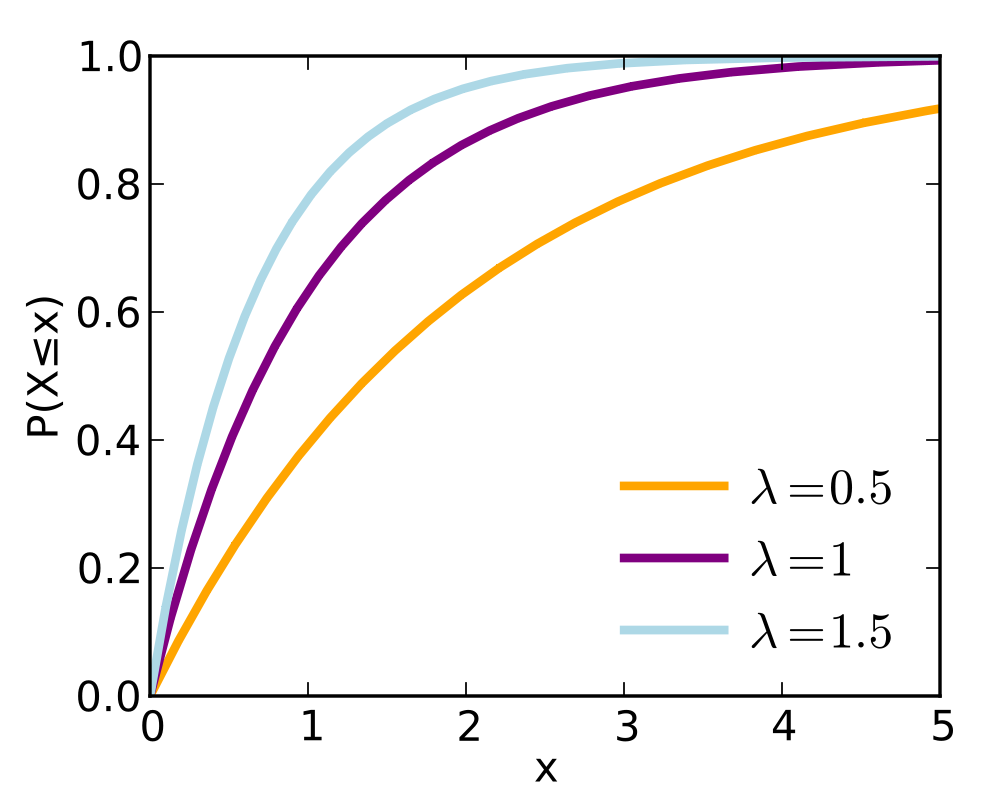
\includegraphics[width=0.5\linewidth]{../Figures/exponentialFunction.png}
  \caption{\label{fig:exponentialFunction} Figure showing the distribution of the equation \ref{eq:distributionFunction}. }
\end{figure}

When $\lambda$ have a value around 0.5, we get a curve \ref{fig:exponentialFunction} which captures how we believe the risk in a network will increase as more non-insured nodes are added. We believe that if one have a growing network consisting of insured nodes only, the first non-insured node added will contribute more risk than the consecutive non-insured nodes. When the 2.nd and 3.rd and so on, node are added there are already a probability that the network will be infected. It reasonable to believe that the overall risk wont increase additive, but at a lower rate. The risk added for each new non-insured node will decrease. Hence we believe that the accentual risk parameter will follow a exponential distribution. 

read more in the paper: Uncertainty in Interdependent Security Games

From this paper follows a description of how to measure risk within a network. The idea is that for a cost $c$, you can protect yourself from threats denoted $p$ outside your own LAN or corporation. However, you can still be affected by threats from non-insured nodes inside the local network. This means that as long as not every node is insured, there will be a risk $q$ for each node not insured. $p$ reflects the probability of getting affected by a risk, and $q$ represents the likelihood of spreading it to others in the local network. The paper presents a swift model for measuring the risk in you local network. The can be used to look at a single nodes utility in the decision of whether to insure or not. 
%appendix

%references



\nocite{*}
\renewcommand*{\bibname}{References}
\bibliographystyle{alpha}
\bibliography{referanser}

%% include here the other chapters
%\begin{appendices}
%\chapter{Analysis}
\section{Analysis of model-2b: Incomplete information}
\label{ch:analysis-of-model-2b}
In this section we present the analysis and mathematics for model 2b: Incomplete information.

When facing a game with incomplete information, there exists two types of equilibriums, one where node 2 is able to seperate node 1's type, called separating equilibrium. The other is where he is not able to separate them, called pooling equilibrium. 
We have two types of node, type 1 $(t1)$: insured and type 2 $(t2)$: not insured. 

\subparagraph{Node 2 is insured.}There are two different games to model, one where node 2 is insured, and the other where he is not insured. We start with the one where he is insured.
Node 1's type is chosen randomly by nature, with probability $p$ of being type 1 and $1-p$ of being type 2.
\begin{figure}[h]
\centering
  \centering
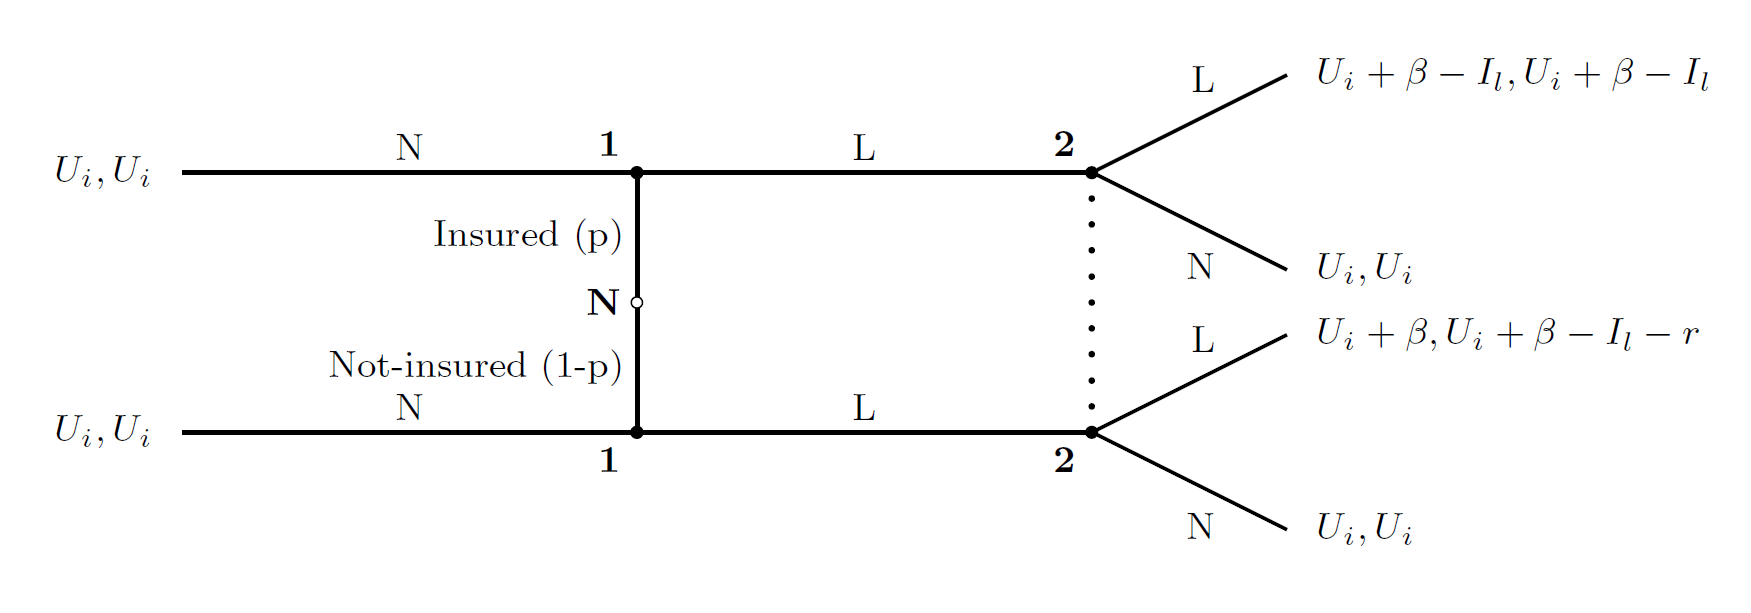
\includegraphics[width=1\linewidth]{../Figures/SignalingGameInsured.png}

\caption{Signalling game with two nodes, node 1's type choosen by nature, node 2 is insured. Node 1 have complete information, node 2 suffer from incomplete information, and act on best response functions based on beliefs. \label{fig:signalingInsured}}

\end{figure}

In the extensive-form shown in Figure \ref{fig:signalingInsured}, we see that $t2's$ strategy L dominates N, and thus $t2$ will never play $N$.
\subparagraph{Separating equilibrium.}
Since node 1 will never play $N$ as type 2, there are only one possible separating equlibrium, type 1 plays $L$ and type 2 plays $N$. Hence node 2's beliefs are as in Eq.(\ref{eq:node2belief}).
\begin{equation}
    \sigma_{1}(t_{i})= 
\begin{cases}
   N,& \text{if } t1\\
   L,& \text{if } t2  
\end{cases}
\label{eq:node2belief}
\end{equation}
Let $\mu_{1}(t_{i} | N )$, denote the probability that node 1 is of type $t_{i}$. By using bayes rule we get this equation:
\begin{equation}
\mu_{1}(t_{1} | N )=\frac{P(N|t_{1})P(t_{1})}{P(N)}=\frac{P(N|t_{1})P(t_{1})}{P(N|t_{1})P(t_{1})+P(N|t_{2})P(t_{2})}
\end{equation}

With node 2's belief, we get that $\mu_{1}(t_{1} | N )=1$ and $\mu_{1}(t_{2} | L )= 1 $. We can now calculate node 2's expected utility from playing L and N:
\begin{eqnarray}
EU_{2}(L,L)=\mu_{1}(t_{1} | L )U_{2}(L,L;t_{1})+\mu_{1}(t_{2} | L )U_{2}(L,L;t_{2}) \nonumber\\
\llap{$\rightarrow$\hspace{50pt}}EU_{2}(L,L)=U_{i}+\beta-I_{l}-r \\
EU_{2}(N,L)=\mu_{1}(t_{1} | L )U_{2}(N,L;t_{1})+\mu_{1}(t_{2} | L )U_{2}(N,L;t_{2})\nonumber\\
\llap{$\rightarrow$\hspace{50pt}}EU_{2}(N,L)=U_{i}
\end{eqnarray}
From these two equations we see that the best response of node 2($BR_2$) when he observes the other node choosing action $L$ is:
\begin{equation}
BR_{2}(L)=
\begin{cases}
L, & \text{if }\beta - r \geq I_{l}\\
N, & \text{if } \beta -r<I_{l}
\end{cases}
\label{eq:insuredBR}
\end{equation}
Node 2's expected utility when type 1 chooses N, is easily seen to be $U_{i}$. 
To confirm if this is a separating equilibrium we must see if node 1 has any incentive to deviate from the strategies in node 2's belief.
Type 2 will never deviate, so lets investigate type 1.
In order to get node 1 to be willing to play N when he knows node 2's best response function, the following must hold: $\beta<I_{l}$. If this is true, then node 2's best response is to play N. I.e. the only separating equilibrium is the following:

\begin{eqnarray}
\beta<I_{l}\\
 \sigma_{1}= 
\begin{cases}
   N,& \text{if } t1\\
   L,& \text{if } t2  
\end{cases}\\
BR_{2}(\sigma_{1})=N
\end{eqnarray} 
This means that in a separating equilibrium, the game will end up with no link establishment.
\subparagraph{Pooling equilibrium.}
In a pooling equilibrium node 2 will not be able to distinguish the two types, and since $t1$'s strategy $L$ dominates $N$, i.e. there is only one possible equilibrium, the one where both types of node 1 plays $L$.
\begin{equation}
    \sigma_{1}(t_{i})= 
\begin{cases}
   L,& \text{if } t1\\
   L,& \text{if } t2  
\end{cases}
\label{eq:node2beliefpooling}
\end{equation}
By using bayes rule we get that $\mu(t_{1}|L)=p$ and $\mu(t_{2}|L)=1-p$.
Node 2's expected utility is then:
\begin{eqnarray}
EU_{2}(L,L)=p(U_{i}+\beta-I_{l})+(1-p)(U_{i}+\beta-I_{l}-r)\nonumber\\
\llap{$\rightarrow$\hspace{50pt}}EU_{2}(L,L)=U_{i}+\beta-I_{l}-r+pr\\
EU_{2}(N,L)=U_{i}
\end{eqnarray}
From this we get node2's best response:
\begin{equation}
BR_{2}(L)=
\begin{cases}
L ,& \text{if } \beta + rp-r\geq I_{l} \\
N ,& \text{if } \beta +rp -r < I_{l} 
\end{cases}
\end{equation}
By using this best response function, node 1 sees that as long as $\beta>I_{l}$ he will never deviate from node 2's beliefs. Hence, it is a pooling equilibrium where both nodes choose $L$, as long as $\beta>I_{l}$ and $\beta +rp-r>I_{l}$.
We also know that: $rp-r\leq0$ is allways true, and thus there also exists a pooling equilibrium where node 1, plays $L$, and node 2, plays $N$. This equilibrium will occur when $\beta>I_{l}$ and $\beta+rp-r<I_{l}$.
\subparagraph{Node 2 not insured.}
Here we will analyze the game when node 2 is not insured.
The rules of the game are as before, the only thing that has changed is the type of node 2, and thus the payoffs are different and we need to see if there exists separating and pooling equilibrium in this game as well.
\begin{figure}[h]
\centering

  \centering
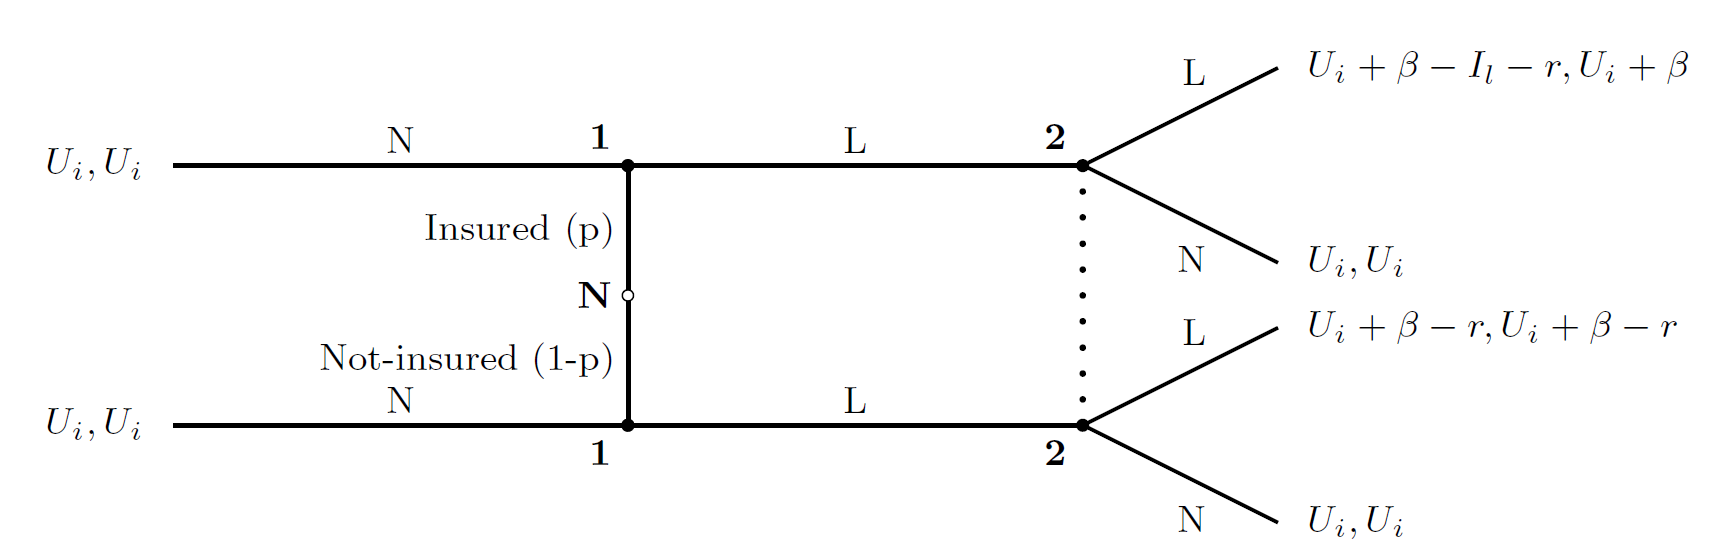
\includegraphics[width=1\linewidth]{../Figures/SignalingGameNotInsured.png}

\caption{Signalling game with two nodes, node 1's type choosen by nature, node2 is not insured. Node 1 have complete information, node 2 suffer from incomplete information, and act on best response functions based on beliefs. \label{fig:signalingNotInsured}}

\end{figure}
\subparagraph{Separating equilibrium.}
In this game there is no dominant strategy for node 1, thus we have to check for the two possible separating equilibriums.
We start with the separating equilibrium with the beliefs shown in Eq.(\ref{eq:node2beliefnotinsured}).
\begin{equation}
    \sigma_{1}(t_{i})= 
\begin{cases}
   L,& \text{if } t1\\
   N,& \text{if } t2  
\end{cases}
\label{eq:node2beliefnotinsured}
\end{equation}
With the beliefs in Eq.(\ref{eq:node2beliefnotinsured}), this is node 2's expected payoffs:
\begin{eqnarray}
EU_{2}(L,L)=(U_{i}+\beta) \\
EU_{2}(N,L)=(U_{i})
\end{eqnarray}
From this we see that his best response when node 1's action is L, is to allways play $L$: \begin{equation}
BR_{2}(L)= L
\end{equation}
To see if this is an equilibrium, we have to see if node 1 has any incentive to deviate. 
We need to check for the two types of node 1:
If $\beta>r$ then type 2 would deviate, because he could achieve a higher payoff by playing $L$, given the beliefs of node 2 in Eq.(\ref{eq:node2beliefnotinsured}). Hence we know that for this to be an equilibrium, the following has to hold
\begin{equation}
\beta < r
\label{eq:sepcondition}
\end{equation}  
When analyzing from node 1 type 1's perspective, for him to play L, this has to hold: $U_{i}+\beta-I_{l}-r > U_{i}$. The only way this can hold is if $\beta>I_{l}+r$. We see that Eq.(\ref{eq:sepcondition}) is violating this condition, and thus we have no separating equilibrium with the beliefs in Eq.(\ref{eq:node2beliefnotinsured}).

Now lets look at the other possible separating equilibrium, see Eq.(\ref{eq:node2beliefnotinsured2}).
\begin{equation}
    \sigma_{1}(t_{i})= 
\begin{cases}
   N,& \text{if } t1\\
   L,& \text{if } t2  
\end{cases}
\label{eq:node2beliefnotinsured2}
\end{equation}
Node 2's expected payoffs are as follows:
\begin{eqnarray}
EU_{2}(L,L)=U_{i}+\beta-r \\
EU_{2}(N,L)=U_{i}
\end{eqnarray}
From this we get the best response function:
\begin{equation}
BR_{2}(L)=
\begin{cases}
L ,& \text{if } \beta\geq r \\
N ,& \text{if } \beta<r 
\end{cases}
\end{equation}
For this to be a separating equilibrium, we need to see if node 1 would deviate from node 2's beliefs. 
Type $t1$ will not deviate as long as $\beta<I_{l}+r$. Type $t2$ will not deviate if $\beta \geq r$, if this condition is true, we see that node 2 will play $L$. I.e. the only separating equilibrium that exists is when node 2 plays $L$, node 1 of type $t1$ plays $N$ and node 1 of type $t2$ plays $L$.
For this to happen we get this condition on $\beta$. \begin{equation}
I_{l}+r>\beta>r
\label{eq:conditionseparatingequilibrium}
\end{equation}
\subparagraph{Pooling equilibrium.}
Two possible, one where both types of node 1 plays $L$, and one where both types plays $N$. Lets first analyze the one where both types of node 1 plays $L$.
\begin{equation}
    \sigma_{1}(t_{i})= 
\begin{cases}
   L,& \text{if } t1\\
   L,& \text{if } t2  
\end{cases}
\label{eq:node2beliefnotinsuredpooling}
\end{equation}
With the beliefs shown above, node 2's expected payoffs are: \begin{eqnarray}
EU_{2}(L)=p(U_{i}+\beta)+(1-p)(U_{i}+\beta-r) \nonumber \\
EU_{2}(L)=U_{i}+\beta-r+pr \\
EU_{2}(N)=U_{i}
\end{eqnarray}
From this we get the best response function :
\begin{equation}
BR_{2}(L)=
\begin{cases}
	L,& \text{if } \beta\geq r-pr\\
   N,& \text{if } \beta<r-pr  
\end{cases}
\end{equation}
Will node 1 deviate knowing this?
Type $t1$ will not deviate as long as: $\beta - I_{l} \geq r$, and type $t2$ will not deviate as long as $\beta >r$.
From this we get the final condition, if $\beta-I_{l}\geq r$ then there exists a pooling equilibrium where both types of node 1 plays $L$ and node 2 also play $L$.
From this we see that the other pooling equilibrium where both types of node 1, plays $N$, will only occur when $\beta<r \text{ and } \beta<I_l+r$.

\chapter{Simulation models}
\section{Model 2: Including parameters}
Here is the Netlogo source code, used to create the simulator for model 2.
 \begin{figure}[htp]\centering{
 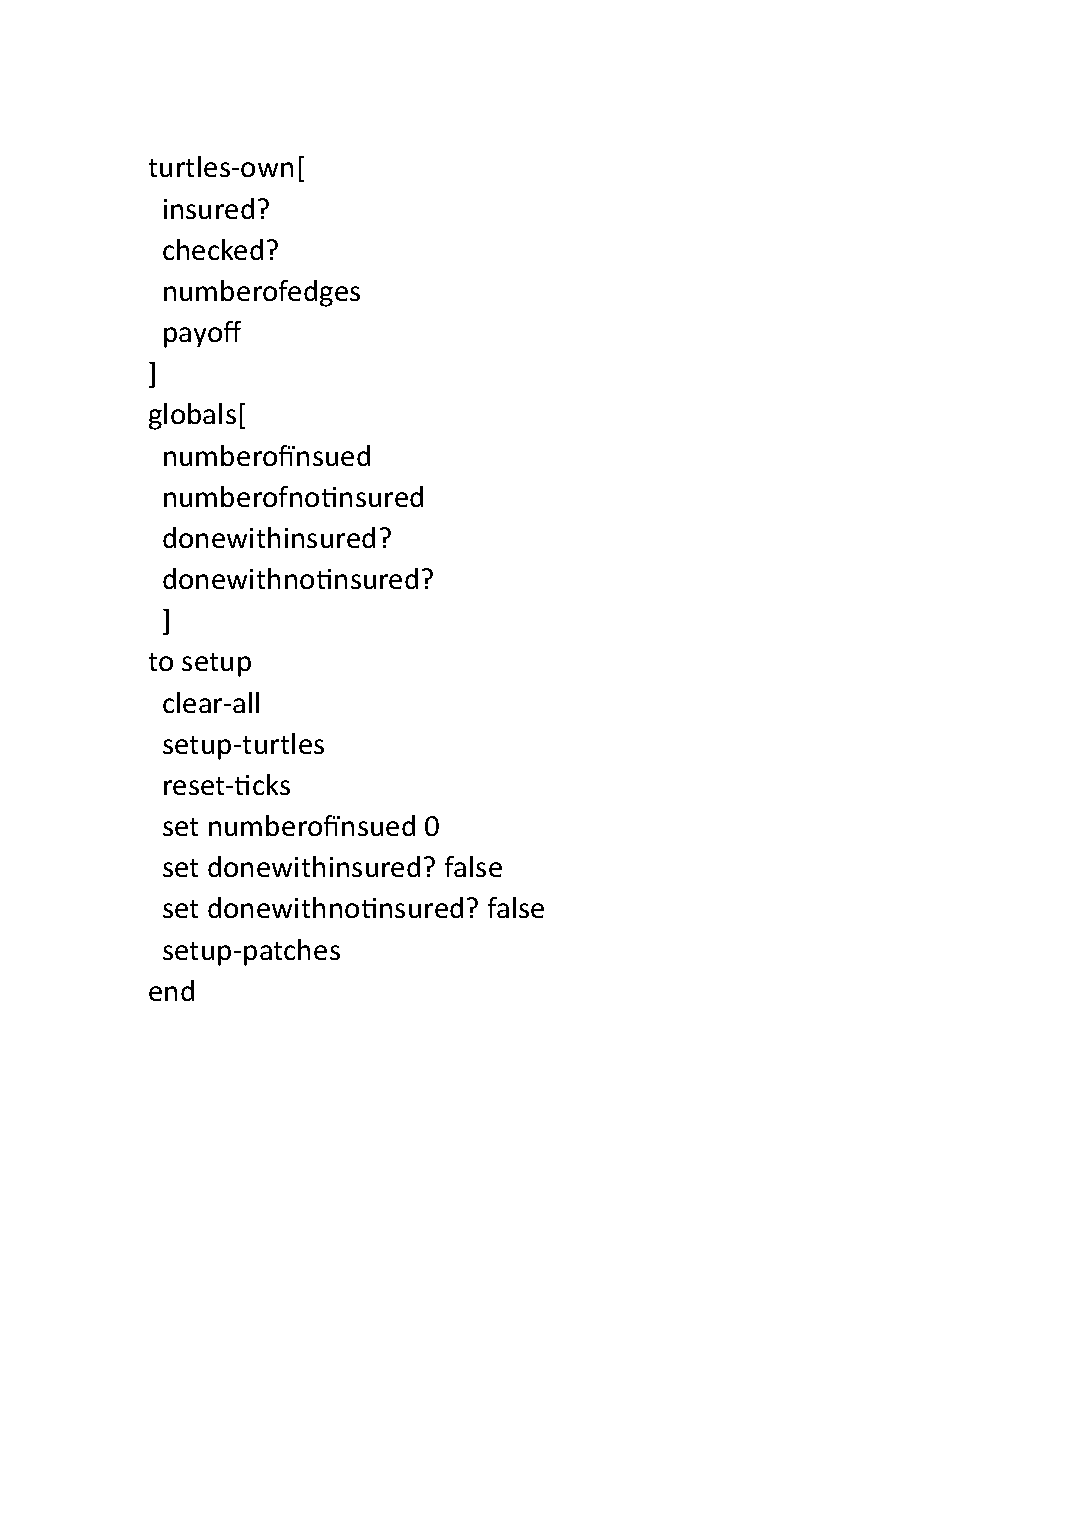
\includepdf[pages=1,scale=0.7,offset=0cm -5cm]{../Figures/Netlogo-model-2.pdf}}
 \end{figure}
 \newpage
 \includepdf[pages=2-3]{../Figures/Netlogo-model-2.pdf}

\section{Model 3: Including maximum node degree and bonus}
Here is the Netlogo source code, used to create the simulator for model 3.
\begin{figure}[htp]\centering{
 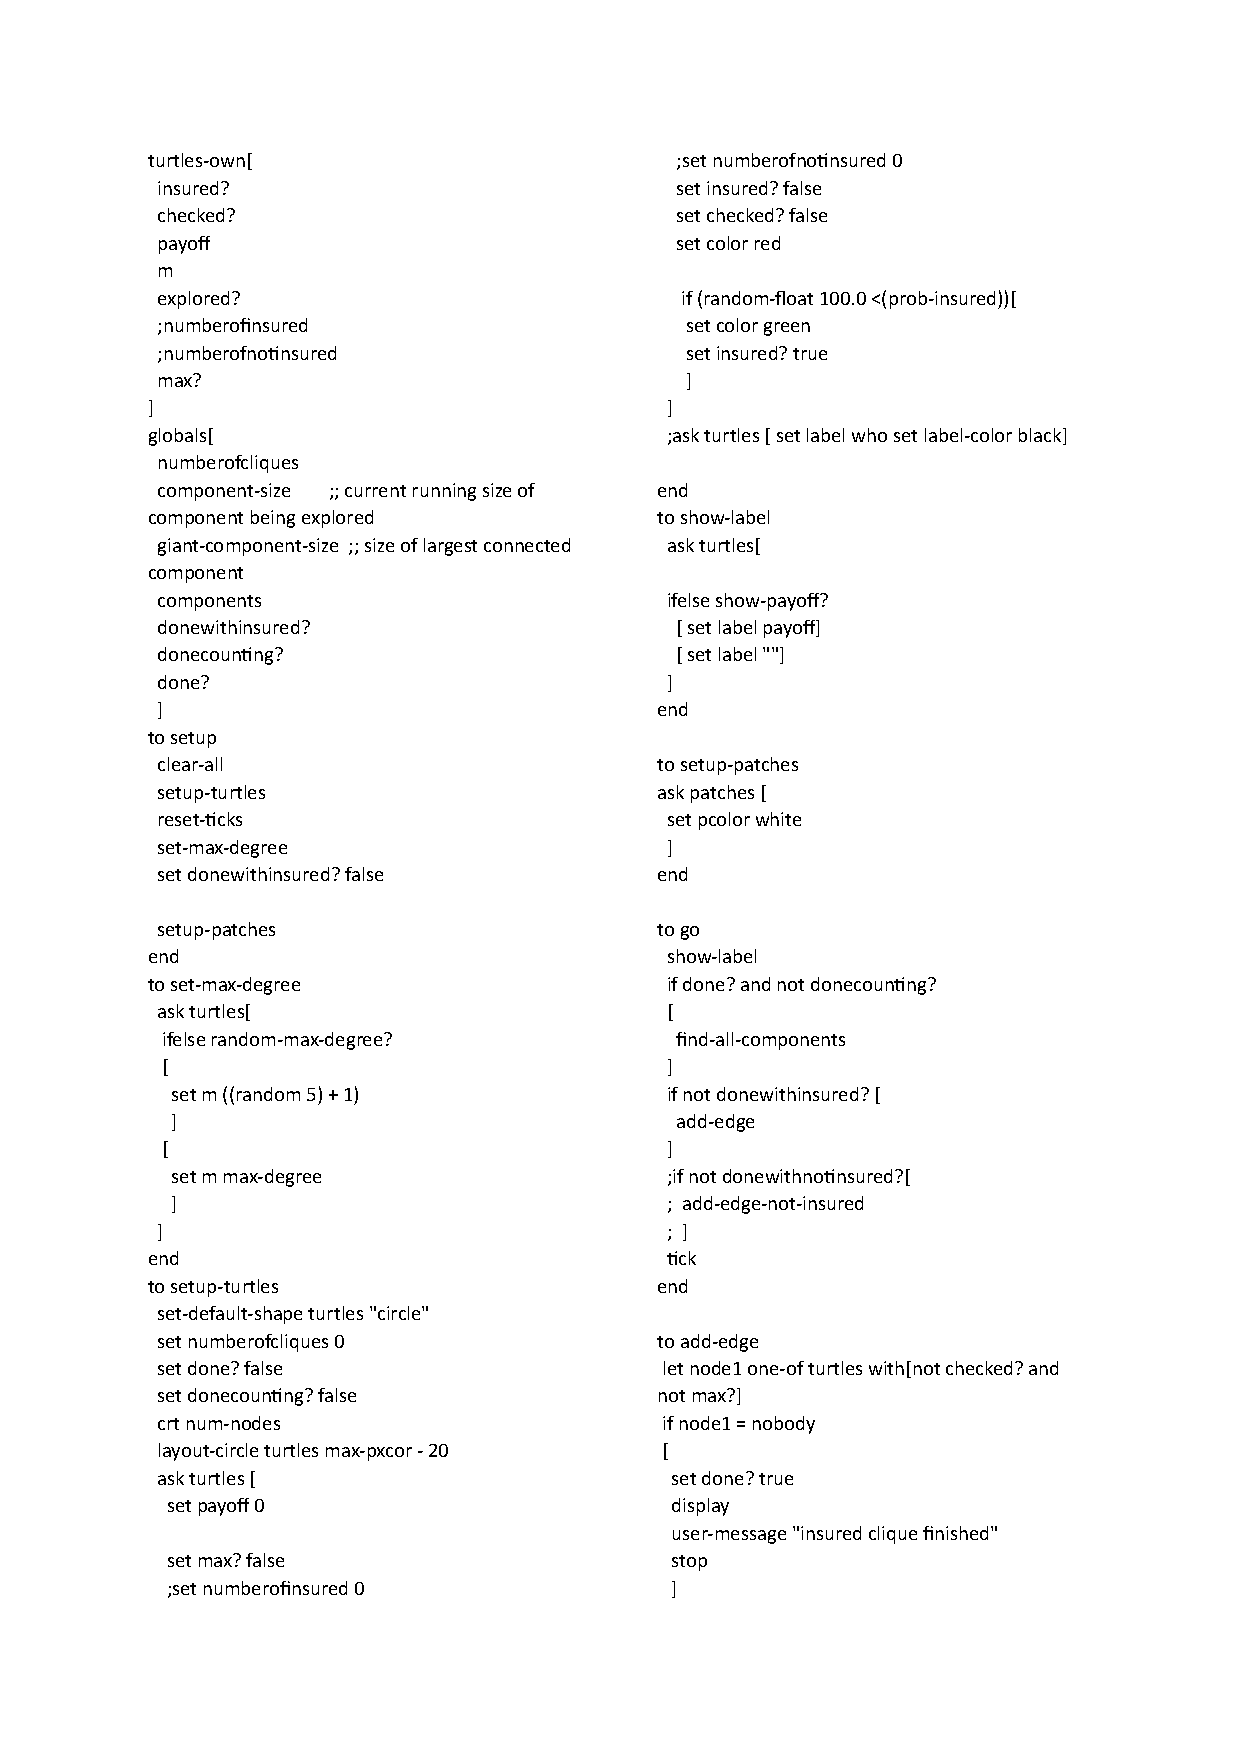
\includepdf[pages=1,scale=0.9,offset=0cm -1cm]{../Figures/Netlogo-model-max-degree.pdf}}
 \end{figure}
 \newpage
 \includepdf[pages=2-4]{../Figures/Netlogo-model-max-degree.pdf}
\section{Model 5: Network externalities}
Here is the Netlogo source code, used to create the simulator for model 5.
\begin{figure}[htp]\centering{
 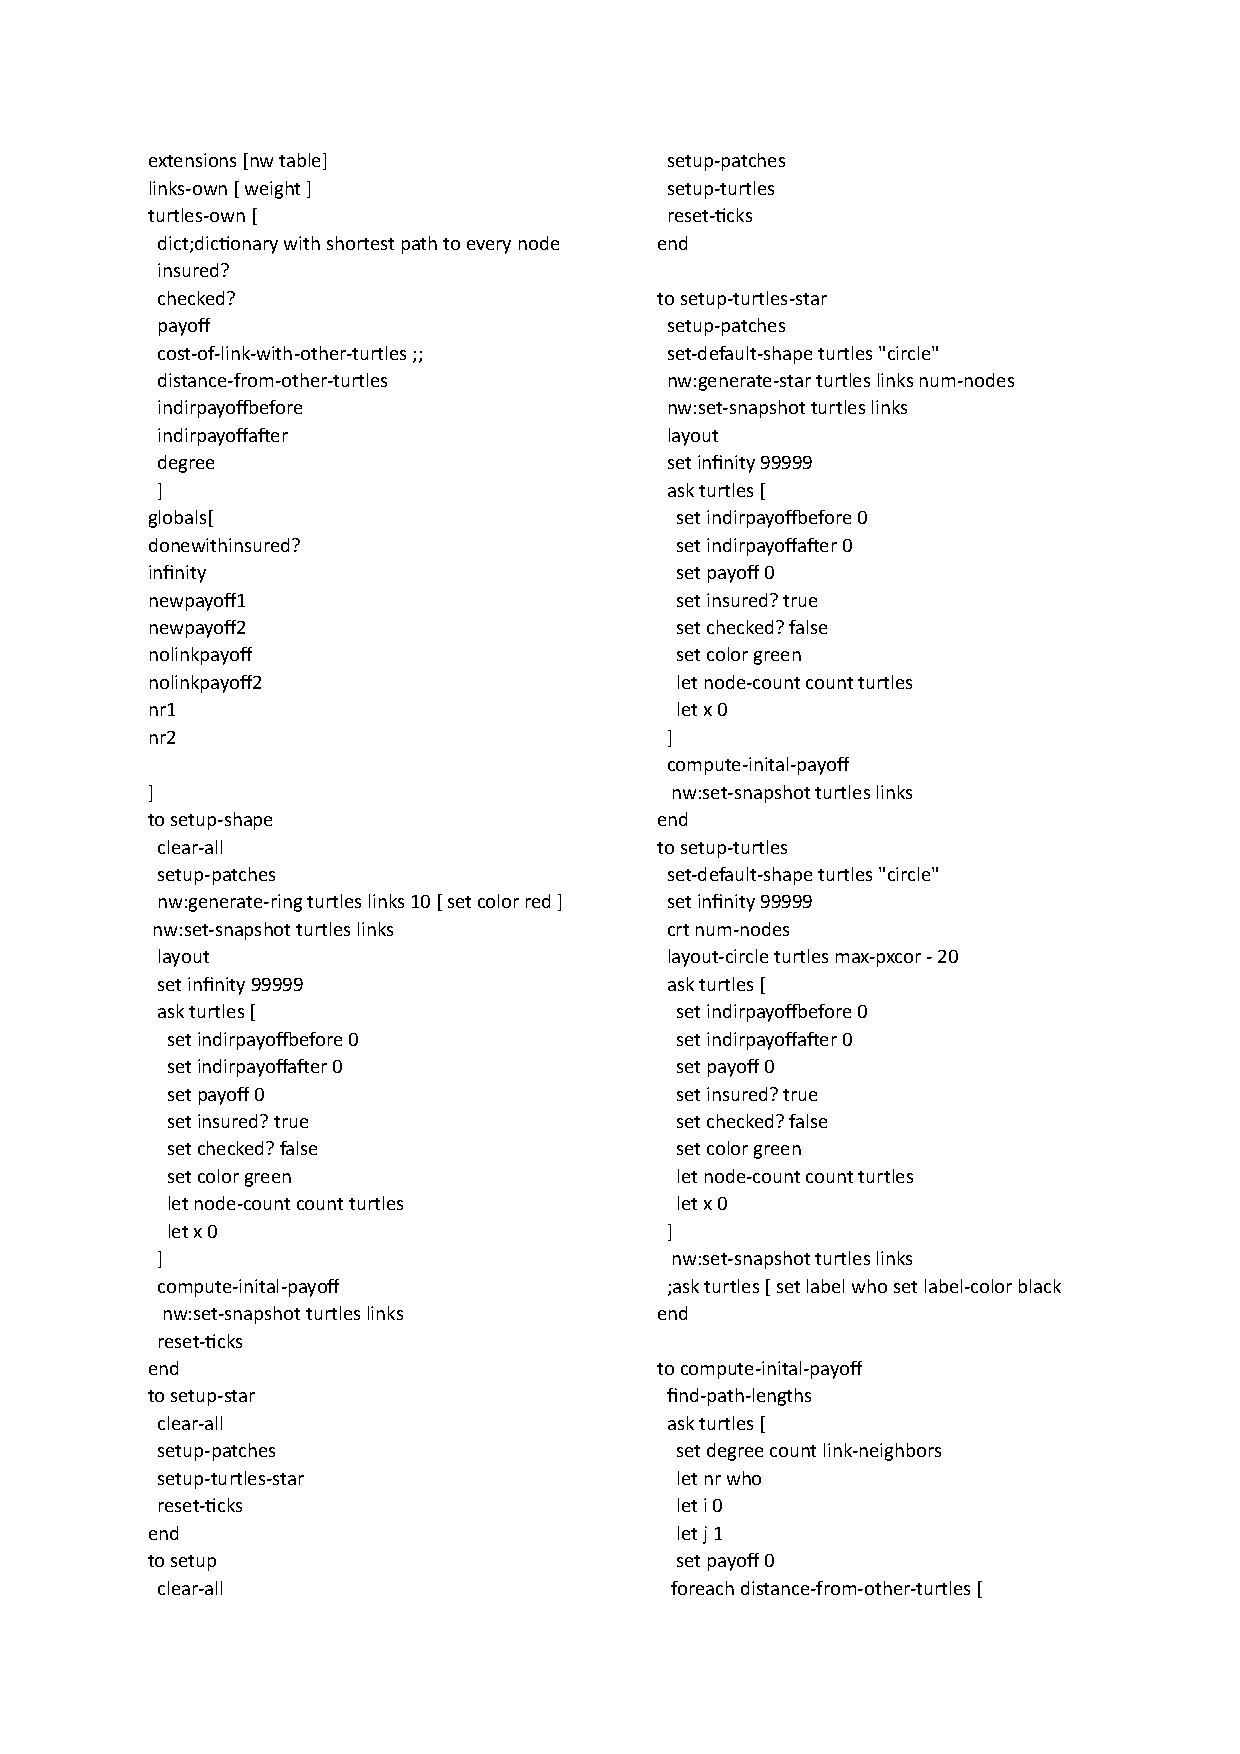
\includepdf[pages=1,scale=0.9,offset=0cm -1cm]{../Figures/Netlogo-model-5.pdf}}
 \end{figure}
 \newpage
 \includepdf[pages=2-4]{../Figures/Netlogo-model-5.pdf}


%\end{appendices}



%% Uncomment the following if you have any appendix
\appendix
 \addtocontents{toc}{%
  \protect\vspace{1em}% 
  \protect\noindent \bfseries \appendixtocname\protect\par
  \protect\vspace{-.5em}%
 }
 \renewcommand{\chaptername}{\appendixname}
%% include below possible appendices (chapters)
\chapter{Analysis}
\section{Analysis of model-2b: Incomplete information}
\label{ch:analysis-of-model-2b}
In this section we present the analysis and mathematics for model 2b: Incomplete information.

When facing a game with incomplete information, there exists two types of equilibriums, one where node 2 is able to seperate node 1's type, called separating equilibrium. The other is where he is not able to separate them, called pooling equilibrium. 
We have two types of node, type 1 $(t1)$: insured and type 2 $(t2)$: not insured. 

\subparagraph{Node 2 is insured.}There are two different games to model, one where node 2 is insured, and the other where he is not insured. We start with the one where he is insured.
Node 1's type is chosen randomly by nature, with probability $p$ of being type 1 and $1-p$ of being type 2.
\begin{figure}[h]
\centering
  \centering
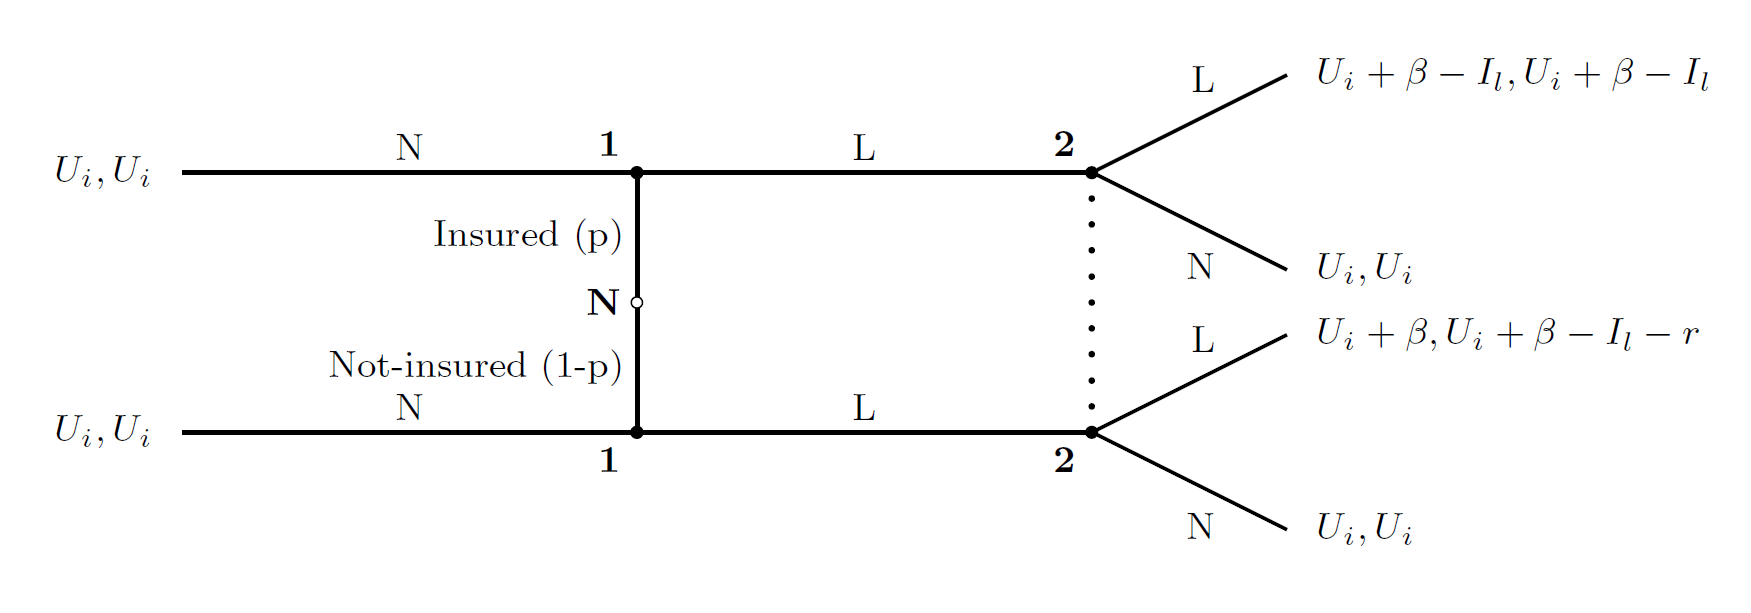
\includegraphics[width=1\linewidth]{../Figures/SignalingGameInsured.png}

\caption{Signalling game with two nodes, node 1's type choosen by nature, node 2 is insured. Node 1 have complete information, node 2 suffer from incomplete information, and act on best response functions based on beliefs. \label{fig:signalingInsured}}

\end{figure}

In the extensive-form shown in Figure \ref{fig:signalingInsured}, we see that $t2's$ strategy L dominates N, and thus $t2$ will never play $N$.
\subparagraph{Separating equilibrium.}
Since node 1 will never play $N$ as type 2, there are only one possible separating equlibrium, type 1 plays $L$ and type 2 plays $N$. Hence node 2's beliefs are as in Eq.(\ref{eq:node2belief}).
\begin{equation}
    \sigma_{1}(t_{i})= 
\begin{cases}
   N,& \text{if } t1\\
   L,& \text{if } t2  
\end{cases}
\label{eq:node2belief}
\end{equation}
Let $\mu_{1}(t_{i} | N )$, denote the probability that node 1 is of type $t_{i}$. By using bayes rule we get this equation:
\begin{equation}
\mu_{1}(t_{1} | N )=\frac{P(N|t_{1})P(t_{1})}{P(N)}=\frac{P(N|t_{1})P(t_{1})}{P(N|t_{1})P(t_{1})+P(N|t_{2})P(t_{2})}
\end{equation}

With node 2's belief, we get that $\mu_{1}(t_{1} | N )=1$ and $\mu_{1}(t_{2} | L )= 1 $. We can now calculate node 2's expected utility from playing L and N:
\begin{eqnarray}
EU_{2}(L,L)=\mu_{1}(t_{1} | L )U_{2}(L,L;t_{1})+\mu_{1}(t_{2} | L )U_{2}(L,L;t_{2}) \nonumber\\
\llap{$\rightarrow$\hspace{50pt}}EU_{2}(L,L)=U_{i}+\beta-I_{l}-r \\
EU_{2}(N,L)=\mu_{1}(t_{1} | L )U_{2}(N,L;t_{1})+\mu_{1}(t_{2} | L )U_{2}(N,L;t_{2})\nonumber\\
\llap{$\rightarrow$\hspace{50pt}}EU_{2}(N,L)=U_{i}
\end{eqnarray}
From these two equations we see that the best response of node 2($BR_2$) when he observes the other node choosing action $L$ is:
\begin{equation}
BR_{2}(L)=
\begin{cases}
L, & \text{if }\beta - r \geq I_{l}\\
N, & \text{if } \beta -r<I_{l}
\end{cases}
\label{eq:insuredBR}
\end{equation}
Node 2's expected utility when type 1 chooses N, is easily seen to be $U_{i}$. 
To confirm if this is a separating equilibrium we must see if node 1 has any incentive to deviate from the strategies in node 2's belief.
Type 2 will never deviate, so lets investigate type 1.
In order to get node 1 to be willing to play N when he knows node 2's best response function, the following must hold: $\beta<I_{l}$. If this is true, then node 2's best response is to play N. I.e. the only separating equilibrium is the following:

\begin{eqnarray}
\beta<I_{l}\\
 \sigma_{1}= 
\begin{cases}
   N,& \text{if } t1\\
   L,& \text{if } t2  
\end{cases}\\
BR_{2}(\sigma_{1})=N
\end{eqnarray} 
This means that in a separating equilibrium, the game will end up with no link establishment.
\subparagraph{Pooling equilibrium.}
In a pooling equilibrium node 2 will not be able to distinguish the two types, and since $t1$'s strategy $L$ dominates $N$, i.e. there is only one possible equilibrium, the one where both types of node 1 plays $L$.
\begin{equation}
    \sigma_{1}(t_{i})= 
\begin{cases}
   L,& \text{if } t1\\
   L,& \text{if } t2  
\end{cases}
\label{eq:node2beliefpooling}
\end{equation}
By using bayes rule we get that $\mu(t_{1}|L)=p$ and $\mu(t_{2}|L)=1-p$.
Node 2's expected utility is then:
\begin{eqnarray}
EU_{2}(L,L)=p(U_{i}+\beta-I_{l})+(1-p)(U_{i}+\beta-I_{l}-r)\nonumber\\
\llap{$\rightarrow$\hspace{50pt}}EU_{2}(L,L)=U_{i}+\beta-I_{l}-r+pr\\
EU_{2}(N,L)=U_{i}
\end{eqnarray}
From this we get node2's best response:
\begin{equation}
BR_{2}(L)=
\begin{cases}
L ,& \text{if } \beta + rp-r\geq I_{l} \\
N ,& \text{if } \beta +rp -r < I_{l} 
\end{cases}
\end{equation}
By using this best response function, node 1 sees that as long as $\beta>I_{l}$ he will never deviate from node 2's beliefs. Hence, it is a pooling equilibrium where both nodes choose $L$, as long as $\beta>I_{l}$ and $\beta +rp-r>I_{l}$.
We also know that: $rp-r\leq0$ is allways true, and thus there also exists a pooling equilibrium where node 1, plays $L$, and node 2, plays $N$. This equilibrium will occur when $\beta>I_{l}$ and $\beta+rp-r<I_{l}$.
\subparagraph{Node 2 not insured.}
Here we will analyze the game when node 2 is not insured.
The rules of the game are as before, the only thing that has changed is the type of node 2, and thus the payoffs are different and we need to see if there exists separating and pooling equilibrium in this game as well.
\begin{figure}[h]
\centering

  \centering
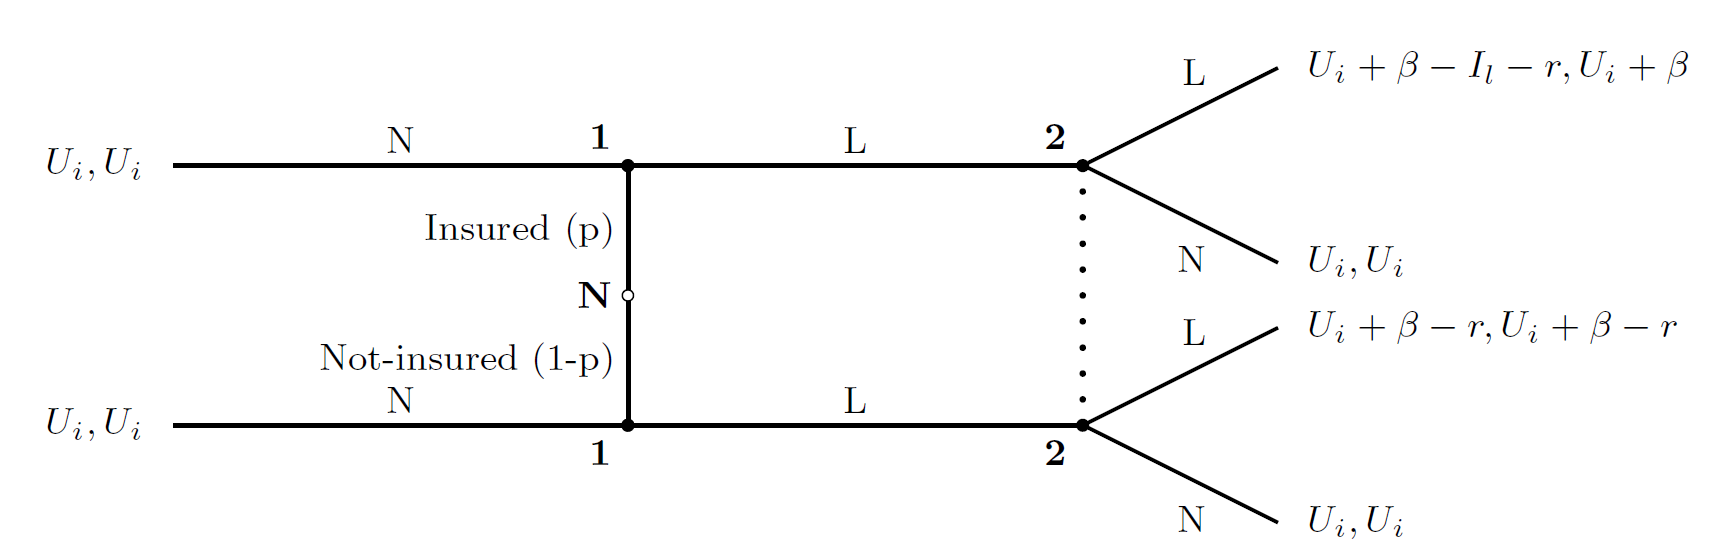
\includegraphics[width=1\linewidth]{../Figures/SignalingGameNotInsured.png}

\caption{Signalling game with two nodes, node 1's type choosen by nature, node2 is not insured. Node 1 have complete information, node 2 suffer from incomplete information, and act on best response functions based on beliefs. \label{fig:signalingNotInsured}}

\end{figure}
\subparagraph{Separating equilibrium.}
In this game there is no dominant strategy for node 1, thus we have to check for the two possible separating equilibriums.
We start with the separating equilibrium with the beliefs shown in Eq.(\ref{eq:node2beliefnotinsured}).
\begin{equation}
    \sigma_{1}(t_{i})= 
\begin{cases}
   L,& \text{if } t1\\
   N,& \text{if } t2  
\end{cases}
\label{eq:node2beliefnotinsured}
\end{equation}
With the beliefs in Eq.(\ref{eq:node2beliefnotinsured}), this is node 2's expected payoffs:
\begin{eqnarray}
EU_{2}(L,L)=(U_{i}+\beta) \\
EU_{2}(N,L)=(U_{i})
\end{eqnarray}
From this we see that his best response when node 1's action is L, is to allways play $L$: \begin{equation}
BR_{2}(L)= L
\end{equation}
To see if this is an equilibrium, we have to see if node 1 has any incentive to deviate. 
We need to check for the two types of node 1:
If $\beta>r$ then type 2 would deviate, because he could achieve a higher payoff by playing $L$, given the beliefs of node 2 in Eq.(\ref{eq:node2beliefnotinsured}). Hence we know that for this to be an equilibrium, the following has to hold
\begin{equation}
\beta < r
\label{eq:sepcondition}
\end{equation}  
When analyzing from node 1 type 1's perspective, for him to play L, this has to hold: $U_{i}+\beta-I_{l}-r > U_{i}$. The only way this can hold is if $\beta>I_{l}+r$. We see that Eq.(\ref{eq:sepcondition}) is violating this condition, and thus we have no separating equilibrium with the beliefs in Eq.(\ref{eq:node2beliefnotinsured}).

Now lets look at the other possible separating equilibrium, see Eq.(\ref{eq:node2beliefnotinsured2}).
\begin{equation}
    \sigma_{1}(t_{i})= 
\begin{cases}
   N,& \text{if } t1\\
   L,& \text{if } t2  
\end{cases}
\label{eq:node2beliefnotinsured2}
\end{equation}
Node 2's expected payoffs are as follows:
\begin{eqnarray}
EU_{2}(L,L)=U_{i}+\beta-r \\
EU_{2}(N,L)=U_{i}
\end{eqnarray}
From this we get the best response function:
\begin{equation}
BR_{2}(L)=
\begin{cases}
L ,& \text{if } \beta\geq r \\
N ,& \text{if } \beta<r 
\end{cases}
\end{equation}
For this to be a separating equilibrium, we need to see if node 1 would deviate from node 2's beliefs. 
Type $t1$ will not deviate as long as $\beta<I_{l}+r$. Type $t2$ will not deviate if $\beta \geq r$, if this condition is true, we see that node 2 will play $L$. I.e. the only separating equilibrium that exists is when node 2 plays $L$, node 1 of type $t1$ plays $N$ and node 1 of type $t2$ plays $L$.
For this to happen we get this condition on $\beta$. \begin{equation}
I_{l}+r>\beta>r
\label{eq:conditionseparatingequilibrium}
\end{equation}
\subparagraph{Pooling equilibrium.}
Two possible, one where both types of node 1 plays $L$, and one where both types plays $N$. Lets first analyze the one where both types of node 1 plays $L$.
\begin{equation}
    \sigma_{1}(t_{i})= 
\begin{cases}
   L,& \text{if } t1\\
   L,& \text{if } t2  
\end{cases}
\label{eq:node2beliefnotinsuredpooling}
\end{equation}
With the beliefs shown above, node 2's expected payoffs are: \begin{eqnarray}
EU_{2}(L)=p(U_{i}+\beta)+(1-p)(U_{i}+\beta-r) \nonumber \\
EU_{2}(L)=U_{i}+\beta-r+pr \\
EU_{2}(N)=U_{i}
\end{eqnarray}
From this we get the best response function :
\begin{equation}
BR_{2}(L)=
\begin{cases}
	L,& \text{if } \beta\geq r-pr\\
   N,& \text{if } \beta<r-pr  
\end{cases}
\end{equation}
Will node 1 deviate knowing this?
Type $t1$ will not deviate as long as: $\beta - I_{l} \geq r$, and type $t2$ will not deviate as long as $\beta >r$.
From this we get the final condition, if $\beta-I_{l}\geq r$ then there exists a pooling equilibrium where both types of node 1 plays $L$ and node 2 also play $L$.
From this we see that the other pooling equilibrium where both types of node 1, plays $N$, will only occur when $\beta<r \text{ and } \beta<I_l+r$.

\chapter{Simulation models}
\section{Model 2: Including parameters}
Here is the Netlogo source code, used to create the simulator for model 2.
 \begin{figure}[htp]\centering{
 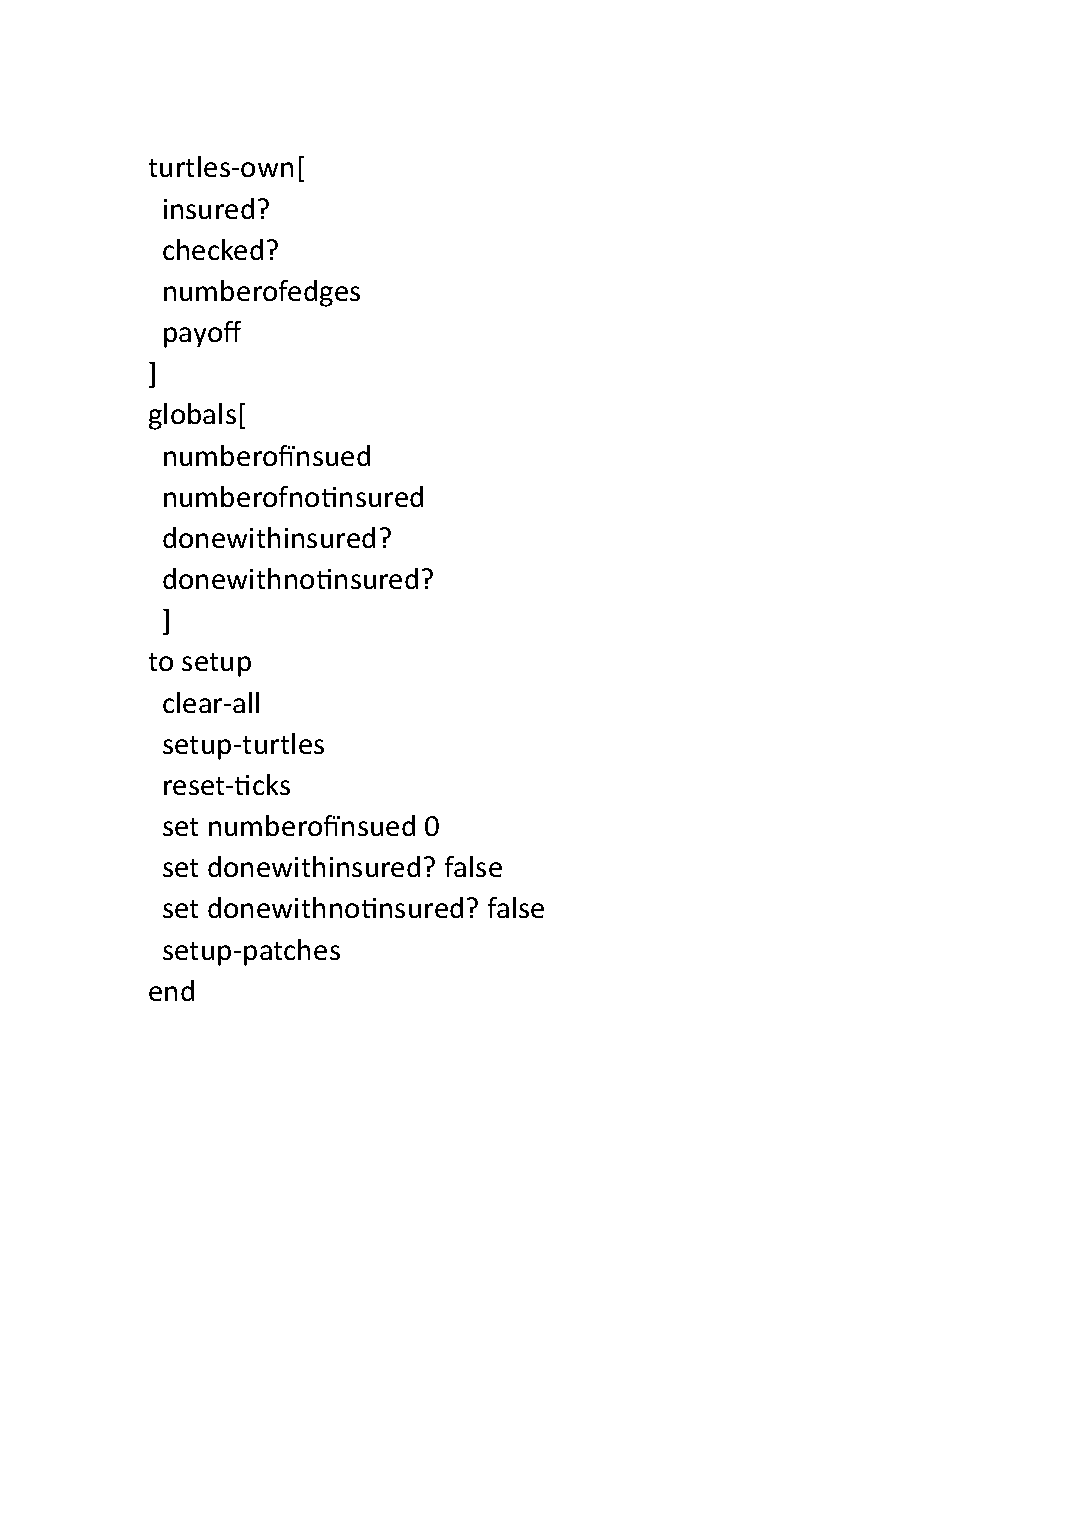
\includepdf[pages=1,scale=0.7,offset=0cm -5cm]{../Figures/Netlogo-model-2.pdf}}
 \end{figure}
 \newpage
 \includepdf[pages=2-3]{../Figures/Netlogo-model-2.pdf}

\section{Model 3: Including maximum node degree and bonus}
Here is the Netlogo source code, used to create the simulator for model 3.
\begin{figure}[htp]\centering{
 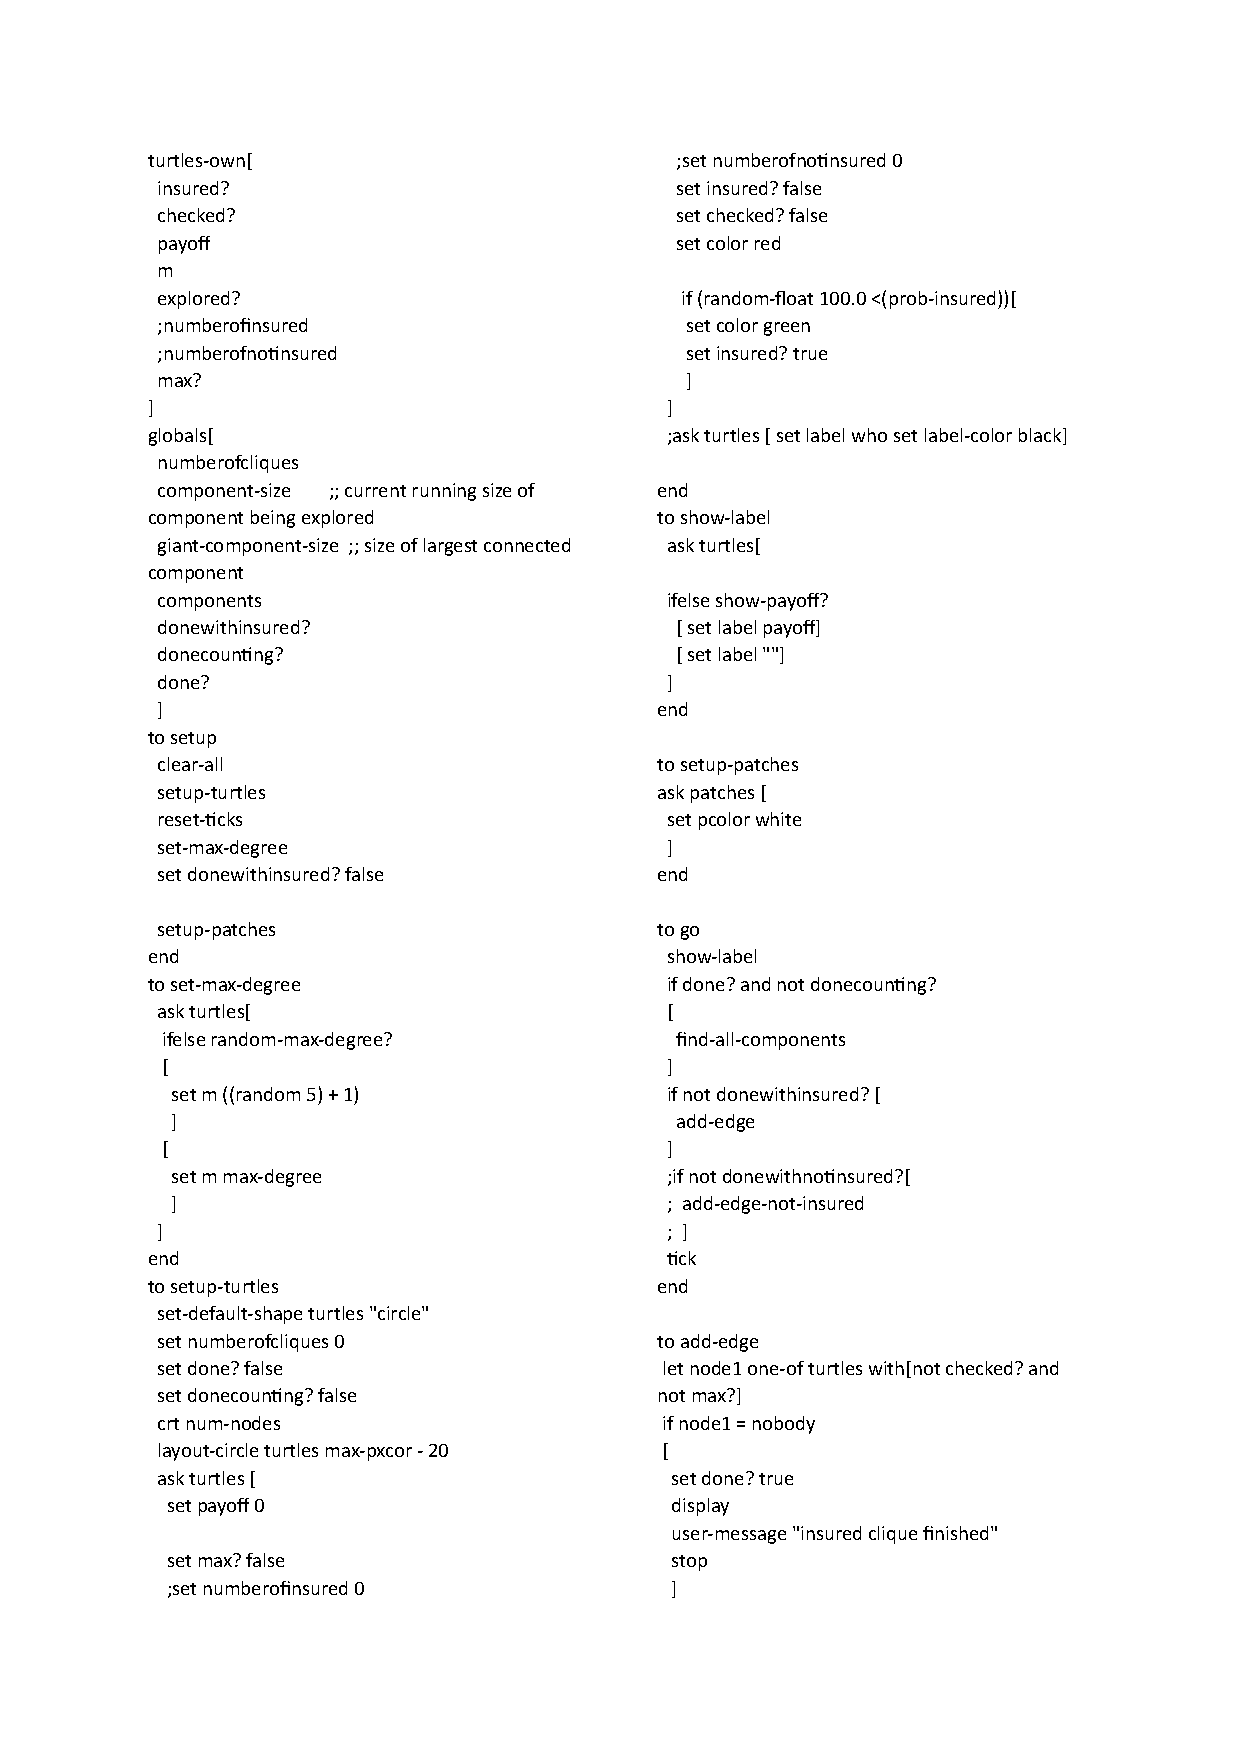
\includepdf[pages=1,scale=0.9,offset=0cm -1cm]{../Figures/Netlogo-model-max-degree.pdf}}
 \end{figure}
 \newpage
 \includepdf[pages=2-4]{../Figures/Netlogo-model-max-degree.pdf}
\section{Model 5: Network externalities}
Here is the Netlogo source code, used to create the simulator for model 5.
\begin{figure}[htp]\centering{
 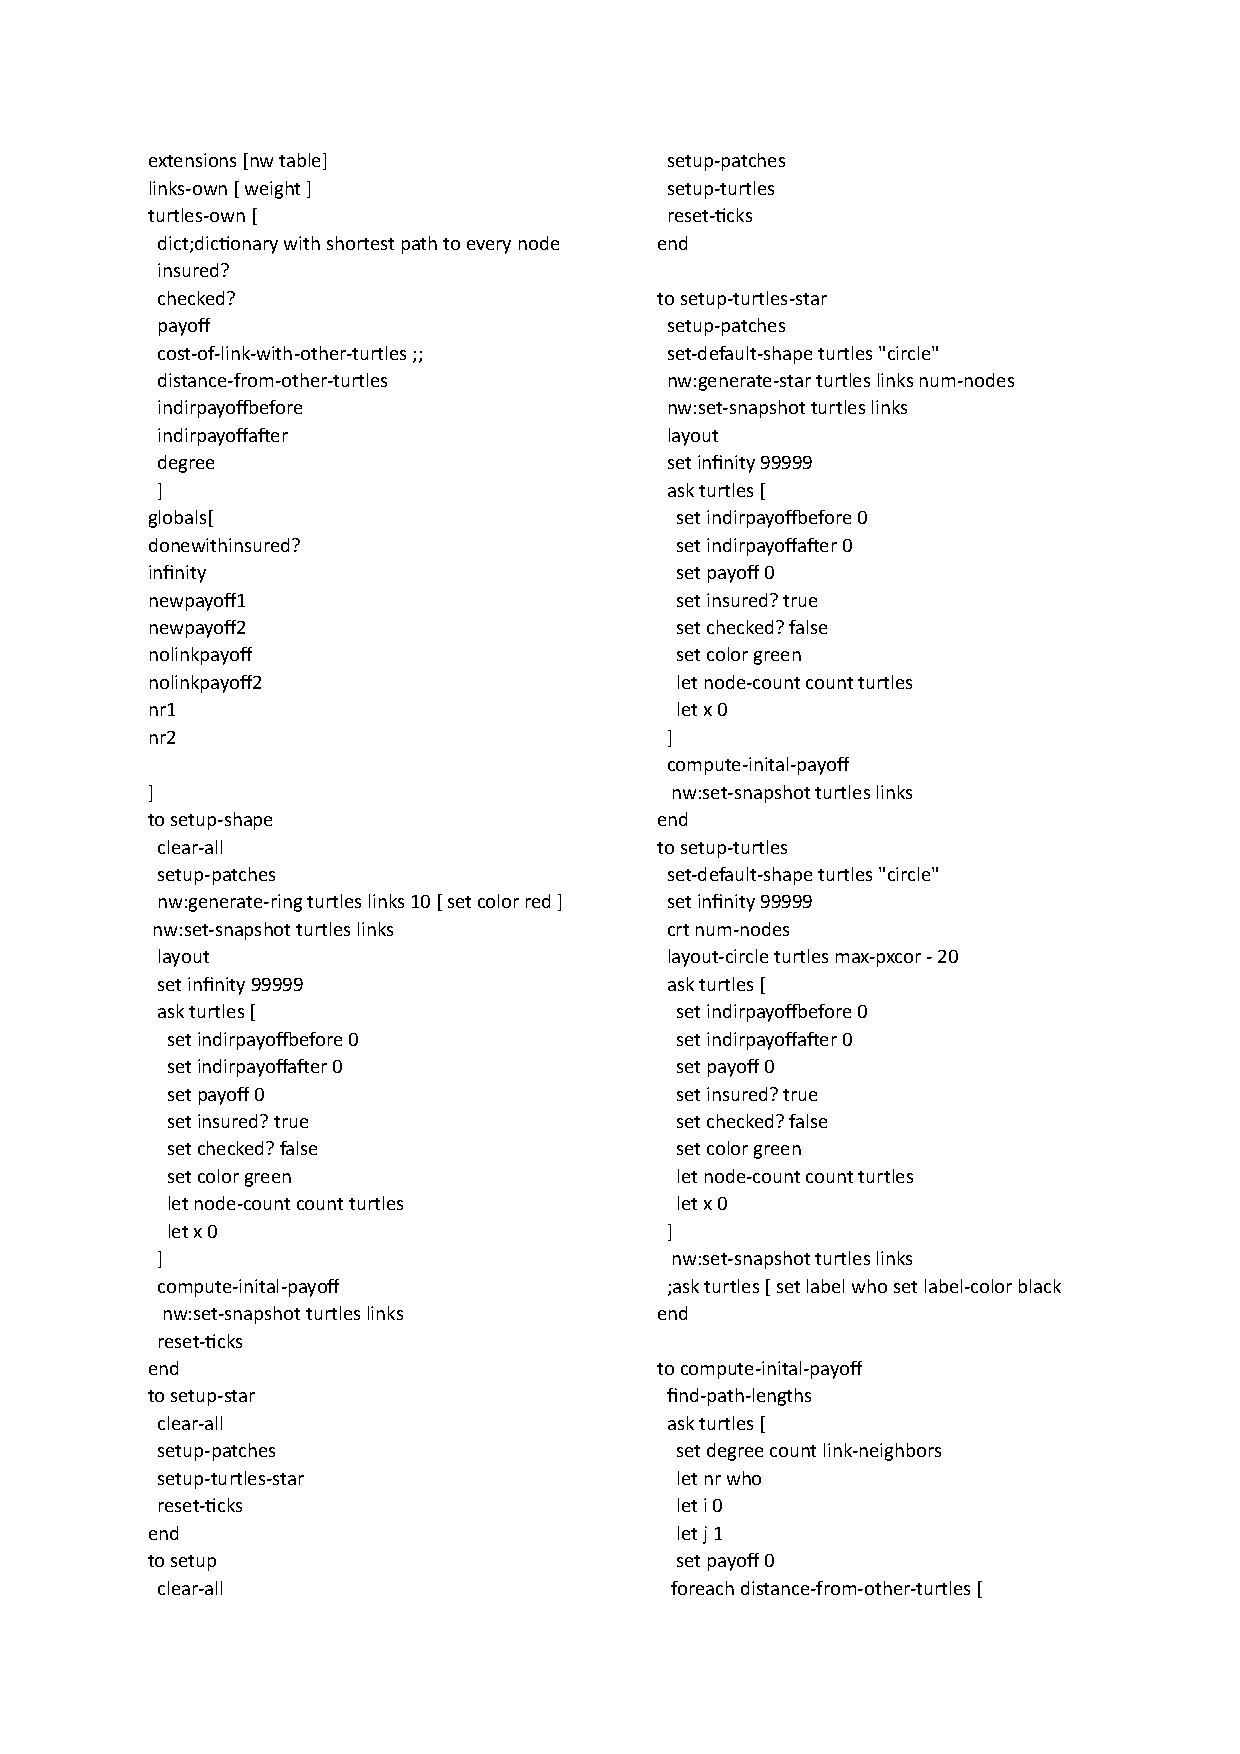
\includepdf[pages=1,scale=0.9,offset=0cm -1cm]{../Figures/Netlogo-model-5.pdf}}
 \end{figure}
 \newpage
 \includepdf[pages=2-4]{../Figures/Netlogo-model-5.pdf}



\end{document} 
